%%%%%%%%%%%%%%%%%%%%%%%%%%%%%%%%%%%%%%%%%%%%%%%%%%%%%%%
%                File: OpEx_style.tex                 %
%             Created: 2 September 2009               %
%                Updated: 15 May 2015                 %
%                                                     %
%           LaTeX template file for use with          %
%           OSA's journals Optics Express,            %
%             Biomedical Optics Express,              %
%            and Optical Materials Express            %
%                                                     %
%  send comments to Theresa Miller, tmiller@osa.org   %
%                                                     %
% This file requires style file, opex3.sty, under     %
	%              the LaTeX article class                %
%                                                     %
%   \documentclass[10pt,letterpaper]{article}         %
%   \usepackage{opex3}                                %
%                                                     %
%                                                     %
%       (c) 2015 Optical Society of America           %
%%%%%%%%%%%%%%%%%%%%%%%%%%%%%%%%%%%%%%%%%%%%%%%%%%%%%%%

%%%%%%%%%%%%%%%%%%%%%%% preamble %%%%%%%%%%%%%%%%%%%%%%%%%%%
\documentclass[10pt,letterpaper]{article}
\usepackage{opex3}
\usepackage{color}
\usepackage{threeparttable}
\usepackage{cite}
\usepackage{subfigure}
\usepackage{float}
\usepackage{amsmath}

%%%%%%%%%%%%%%%%%%%%%%% begin %%%%%%%%%%%%%%%%%%%%%%%%%%%%%%
\begin{document}

\title{High-order harmonic generation in polar media induced by chirped few-cycle pulses}

\author{Pidong Hu,$^1$ Yueping Niu,$^{1,3}$ Shangqing Gong,$^{1,4}$  and Chengpu Liu$^{2,*}$}

\address{$^1$Department of Physics, East China University of Science and Technology, \\
Meilong Road 130, Shanghai 200237, China\\
$^2$State Key Laboratory of High Field Laser Physics, Shanghai Institute of Optics and Fine Mechanics, Chinese Academy of Sciences, Qinghe Road 390, Shanghai 201800, China\\
$^{3}$niuyp@ecust.edu.cn\\
$^{4}$sqgong@ecust.edu.cn
}

\email{*chpliu@siom.ac.cn}

% \homepage{http:...} %% author's URL, if desired

%%%%%%%%%%%%%%%%%%% abstract and OCIS codes %%%%%%%%%%%%%%%%
%% [use \begin{abstract*}...\end{abstract*} if exempt from copyright]

\begin{abstract}
The high-order harmonic generation in a polar medium ( a medium with a permanent dipole moment) driven by a chirped few-cycle laser pulse is investigated via numerically solving the nonlinear Bloch equations or Maxwell-Bloch equations if taking the propagation effect into account. The time-frequency characteristic of the harmonic is analyzed by means of the wavelet transform to induced time-dependent dipole moment. The simulation results demonstrate that, the harmonic cutoff energy can be dramatically extended as a result of the existence of the permanent dipole moment, and the quantum trajectory number for plateau harmonics can be largely reduced due to the introduce of chirps to the laser driver. Consequently, an attosecond pulse pair (APP) is generated instead of a general attosecond pulse train. In addition, the propagation effect can make the APP's intensity enhanced by one order at a suitable propagation distance with small duration broadening, and the enhancement process can be modulated by changing the medium's density.
\end{abstract}

\ocis{(140.7090) Ultralfast lasers; (190.4180) Multiphoton processes; (320.7110) Ultrafast nonlinear optics; (190.5530) Pulse propagation and solitons.} % REPLACE WITH CORRECT OCIS CODES FOR YOUR ARTICLE, MINIMUM OF TWO; Avoid using the OCIS codes for “General” or “General science” whenever possible.
%For a complete list of OCIS codes, visit: http://www.opticsinfobase.org/submit/ocis/

%%%%%%%%%%%%%%%%%%%%%%% References %%%%%%%%%%%%%%%%%%%%%%%%%
%%%%%%%%%%%%%%%%%%%%%%% References %%%%%%%%%%%%%%%%%%%%%%%%%
\begin{thebibliography}{99}
\bibitem{Mokhtari-chemical-bond-Nature-1990}A. Mokhtari, P. Cong, J. L. Herek, and A. H. Zewail, ``Direct femtosecond mapping of trajectories in a chemical reaction," \nat {\bf 348}, 225--227 (1990).

\bibitem{Ergler-Vibration-PRL-2006}T. Ergler, B. Feuerstein, A. Rudenko, K. Zrost, C. D. Schr\"{o}ter, R. Moshammer, and J. Ullrich, ``Quantum-phase resolved mapping of ground-state vibrational ${\rm{D}}_{2}$ wave packets via selective depletion in intense laser pulses," \prl {\bf 97}, 103004 (2006).

\bibitem{Uiberacker-Attosecond-real-time-Nature-2007}M. Uiberacker, T. Uphues, M. Schultze, A. J. Verhoef, V. Yakovlev, M. F. Kling, J. Rauschenberger, N. M. Kabachnik, H. Schroder, M. Lezius, K. L. Kompa, H. G. Muller, M. J. J. Vrakking, S. Hendel, U. Kleineberg, U. Heinzmann, M. Drescher, and F. Krausz, ``Attosecond real-time observation of electron tunnelling in atoms," \nat {\bf 446}, 627--632 (2007).

\bibitem{Krausz-Attosecon-Review-2009}F. Krausz and M. Ivanov, ``Attosecond physics," \rmp {\bf 81}, 163--234 (2009).

\bibitem{Chang2012-OL-67as}K. Zhao, Q. Zhang, M. Chini, Y. Wu, X. Wang, and Z. Chang, ``Tailoring a 67 attosecond pulse through advantageous phase-mismatch," \ol {\bf 37}(18), 3891--3893 (2012).

\bibitem{Shore-HHG-Origin-JPB-1987}B. W. Shore and P. L. Knight, ``Enhancement of high optical harmonics by excess-photon ionisation," J. Phys. B: At. Mol. Opt. Phys. {\bf 20}, 413 (1987).

\bibitem{McPherson-Early-HHG-JOSAB-1987}A. McPherson, G. Gibson, H. Jara, U. Johann, T. S. Luk, I. A. McIntyre, K. Boyer, and C. K. Rhodes, ``Studies of multiphoton production of vacuum-ultraviolet radiation in the rare gases," \josab {\bf 4}, 595--601 (1987).

\bibitem{Ferray-Early-HHG-JPB-1988}M. Ferray, A. L'Huillier, X. F. Li, L. A. Lompre, G. Mainfray, and C. Manus, ``Multiple-harmonic conversion of 1064 nm radiation in rare gases," J. Phys. B: At. Mol. Opt. Phys. {\bf 21}, L31 (1988).

\bibitem{Corkum-PRL-1993}P. B. Corkum, ``Plasma perspective on strong field multiphoton ionization," \prl {\bf 71}, 1994--1997 (1993).

\bibitem{Lewenstein-SFA-PRA-1994}M. Lewenstein, P. Balcou, M. Y. Ivanov, A. L'Huillier, and P. B. Corkum, ``Theory of high-harmonic generation by low-frequency laser fields," \pra {\bf 49}, 2117--2132 (1994).

\bibitem{1997Review}M. Protopapas, C. H. Keitel, and P. L. Knight, ``Atomic physics with super-high intensity lasers," Rep. Prog. Phys. {\bf 60}, 389--486 (1997).

\bibitem{Sundaram-Early-Two-Level-PRA-1990}B. Sundaram and P. W. Milonni, ``High-order harmonic generation: simplified model and relevance of single-atom theories to experiment," \pra {\bf 41}, 6571--6573 (1990).

\bibitem{Ivanov-Early-Two-Level-PRA-1993}M. Y. Ivanov and P. B. Corkum, ``Generation of high-order harmonics from inertially confined molecular ions," \pra {\bf 48}, 580--590 (1993).

\bibitem{Kaplan-Early-Two-Level-PRA-1994}A. E. Kaplan and P. L. Shkolnikov, ``Superdressed two-level atom: very high harmonic generation and multiresonances," \pra {\bf 49}, 1275--1280 (1994).

\bibitem{Gauthey-Early-Two-Level-PRA-1997}F. I. Gauthey, B. M. Garraway, and P. L. Knight, ``High harmonic generation and periodic level crossings," \pra {\bf 56}, 3093--3096 (1997).

\bibitem{Faria-Two-Level-Three-Step-PRA-2002}C. Figueira de Morisson Faria and I. Rotter, ``High-order harmonic generation in a driven two-level atom: periodic level crossings and three-step processes," \pra {\bf 66}, 013402 (2002).

\bibitem{Sansone-Polarization-gate-Nature-2006}G. Sansone, E. Benedetti, F. Calegari, C. Vozzi, L. Avaldi, R. Flammini, L. Poletto, P. Villoresi, C. Altucci, R. Velotta, S. Stagira, S. De Silvestri, and M. Nisoli, ``Isolated single-cycle attosecond pulses," Science {\bf 314}, 443--446 (2006).

\bibitem{Carrera-Chirp-PRA-2007}J. J. Carrera and S.-I. Chu, ``Extension of high-order harmonic generation cutoff via coherent control of intense few-cycle chirped laser pulses," \pra {\bf 75}, 033807 (2007).

\bibitem{ZengZhinan-Two-Color-PRL-2007}Z. Zeng, Y. Cheng, X. Song, R. Li, and Z. Xu, ``Generation of an extreme ultraviolet supercontinuum in a two-color laser field," \prl {\bf 98}, 203901 (2007).

\bibitem{ChangZenghu-Combination-PRA-2007}Z. Chang, ``Controlling attosecond pulse generation with a double optical gating," \pra {\bf 76}, 051403 (2007).

\bibitem{Gong-Two-Level-Two-Color-JMO-1999}S. Gong, Z. Wang, S. Du, and Z. Xu, ``Coherent control of high-order harmonic generation in a two-level atom driven by intense two-colour laser fields," \jmo {\bf 46}, 1669--1676 (1999).

\bibitem{WANG-ZHONG-YANG-Two-Level-Attosecond-generation-1999}Z. Wang, S. Gong, and Z. Xu, ``Attosecond light pulse generation in a strongly driven two-level atom," Acta Phys. Sin. {\bf 48}, 961--965 (1999).

\bibitem{LiuChengpu-Two-Level-PRA-2004}C. Liu, S. Gong, R. Li, and Z. Xu, ``Coherent control in the generation of harmonics and hyper-Raman lines from a strongly driven two-level atom," \pra {\bf 69}, 023406 (2004).

\bibitem{YangWeifeng-Two-Level-PLA-2007}W. Yang, S. Gong, R. Li and Z. Xu, ``Generation of attosecond pulses in a system with permanent dipole moment," Phys. Lett. A {\bf 362}, 37--41 (2007).

\bibitem{CuiNi2010NJP-wavelet}N. Cui, Y. Xiang, Y. Niu, and S. Gong, ``Coherent control of terahertz harmonic generation by a chirped few-cycle pulse in a quantum well," New J. Phys. {\bf 12}, 013009 (2010).

\bibitem{IAP-reference1-1998}Le Kien, Fam Midorikawa, Katsumi Suda, and Akira, ``Attosecond pulse generation using high harmonics in the multicycle regime of the driver pulse," \pra {\bf 58}(4), 3311--3319 (1998).

\bibitem{IAP-reference2-2008}Yongli Yu, Xiaohong Song, Yuxi Fu, Ruxin Li, Ya Cheng, and Zhizhan Xu, ``Theoretical investigation of single attosecond pulse generation in an orthogonally polarized two-color laser field," \opex {\bf 16}(2), 686--694 (2008).

\bibitem{IAP-reference3-2008}Qingbin Zhang, Peixiang Lu, Pengfei Lan, Weiyi Hong, and Zhenyu Yang, ``Multi-cycle laser-driven broadband supercontinuum with a modulated polarization gating," \opex {\bf 16}(13), 9795--9803 (2008).

\bibitem{IAP-reference4-2012}Yang Xiang, Yueping Niu, and Shangqing Gong, ``Proposal for isolated-attosecond-pulse generation in the multicycle regime through modulation of the carrier wave," \pra {\bf 85}(2), 023808 (2012).

\bibitem{attochirp-ref1-2003}Y. Mairesse, A. de Bohan, L. J. Frasinski, H. Merdji, L. C. Dinu, P. Monchicourt, P. Breger, M. Kova\v{c}ev, R. Ta\"{i}eb, B. Carr\'{e}, H. G. Muller, P. Agostini, and P. Sali\`{e}res,  ``Attosecond synchronization of high-harmonic soft X-rays," Science {\bf 302}, 1540--1543 (2003).

\bibitem{attochirp-ref2-2007}J. Tate, T. Auguste, H. G. Muller, P. Sali\`{e}res, P. Agostini, and L. F. DiMauro, ``Scaling of wave-packet dynamics in an intense midinfrared field," \prl {\bf 98}(1), 013901 (2007).

\bibitem{attochirp-ref3-2009}G. Doumy, J. Wheeler, C. Roedig, R. Chirla, P. Agostini, and L. F. DiMauro, ``Attosecond synchronization of high-order harmonics from midinfrared drivers," \prl {\bf 102}(9), 093002 (2009).

\bibitem{2009Review}P. Sali\`{e}res and I. Christov, ``Macroscopic effects in high-order harmonic generation," in \emph{Strong Field Laser Physics}, Thomas Brabec, ed. (Springer, 2009).

\bibitem{Kalosha-Two-Level-PRL-1999}V. P. Kalosha and J. Herrmann, ``Formation of optical subcycle pulses and full Maxwell-Bloch solitary waves by coherent propagation effects," \prl {\bf 83}, 544--547 (1999).

\bibitem{Ziolkowski-Two-Level-Method-PRA-1995}R. W. Ziolkowski, J. M. Arnold, and D. M. Gogny, ``Ultrafast pulse interactions with two-level atoms," \pra {\bf 52}, 3082--3094 (1995).


%\begin propagation references
\bibitem{Pan-Ruiqin-Permanent-dipole-moment-2011}R. Pan, ``Few-cycle ultrashort pulse laser propagation in organic molecular material," Acta Sinica Quantum Optica {\bf 17}, 52--57 (2011).

\bibitem{Xiao-Jian-PRA-2002}J. Xiao, Z. Wang, and Z. Xu, ``Area evolution of a few-cycle pulse laser in a two-level-atom medium," \pra {\bf 65}, 031402 (2002).

\bibitem{Xia-Keyu-OE-2005}K. Xia, S. Gong, C. Liu, X. Song, and Y. Niu, ``Near dipole-dipole effects on the propagation of few-cycle pulse in a dense two-level medium," \opex {\bf 13}, 5913--5924 (2005).

%\end propagation references

\bibitem{MyOE2013}P. Hu, Y. Niu, Y. Xiang, and S. Gong, ``Above-threshold ionization by few-cycle phase jump pulses," \opex {\bf 21}, 24309--24317 (2013).

\bibitem{MyOE2015}P. Hu, Y. Niu, Y. Xiang, S. Gong, and C. Liu, ``Carrier-envelope phase dependence of molecular harmonic spectral minima induced by mid-infrared laser pulses," \opex {\bf 21}(20), 24309--24317 (2015).

\bibitem{TongXiaoMin2000PRA-Wavelet}X.-M. Tong and S.-I. Chu, ``Probing the spectral and temporal structures of high-order harmonic generation in intense laser pulses," \pra {\bf 61}, 021802(R) (2000).

\bibitem{Yee}K. S. Yee, ``Numerical solution of initial boundary value problems involing Maxwell's equations in isotropic media," \aprop {\bf 14}, 302--307 (1966).

\bibitem{Mur-Absorption}G. Mur, ``Absorbing boundary conditions for the finite-difference approximation of the time-domain electromagnetic-field equations," IEEE. Trans. Electronmagn. Compat. {\bf EMC-23}, 377--382 (1981).

\bibitem{Chirp-Reference-2013PRA}P. Kumar and A. K. Sarma, ``Ultrafast and selective coherent population transfer in four-level atoms by a single nonlinearly chirped femtosecond pulse," \pra {\bf 88}(3), 033823 (2013).
	
\end{thebibliography}

%%%%%%%%%%%%%%%%%%%%%%%%%%  body  %%%%%%%%%%%%%%%%%%%%%%%%%%
\section{Introduction}
Femtosecond laser technology has obtained rapid development over the past decades, and it provides us important tools to study the strong-filed physics as well as the ultrafast phenomena. People can observe the ultra-fast dynamic chemical reaction process using the femtosecond technology, such as, the breaking and restructuring of the chemical bond \cite{Mokhtari-chemical-bond-Nature-1990} and the vibrations of an atom or a molecule \cite{Ergler-Vibration-PRL-2006}. However, if we want to observe further faster physical phenomena, such as electron motivation, a sub-femtosecond or attosecond pulse should be used \cite{Uiberacker-Attosecond-real-time-Nature-2007}. In recent decades, one important and effective solution to generate attosecond laser pulse is the Fourier synthesis to the high-order harmonics. Krausz's team has first obtained the sub-femtosecond pulse output (650 as) experimentally in 2002 \cite{Krausz-Attosecon-Review-2009}. From then on, two milestones are obtained: one is that Krausz's team \cite{Krausz-Attosecon-Review-2009} obtained an 80 as pulse by utilizing a 3.3 fs driving laser pulse, which broke the limit of 100 as, and the other is Chang's group composed a 67 as single isolated attosecond pulse from an extreme UV supercontinuum \cite{Chang2012-OL-67as}.

As for the high-order harmonic generation (HHG ), it is first proposed by Shore and Knight in 1987 \cite{Shore-HHG-Origin-JPB-1987}, and subsequently, observed experimentally by McPherson \cite{McPherson-Early-HHG-JOSAB-1987} and Farray \cite{Ferray-Early-HHG-JPB-1988}. Its intuitive physical mechanism can be summarized as a \emph{three-step} model proposed by Corkum first \cite{Corkum-PRL-1993} and developed by Lewenstein \emph{et al.} later\cite{Lewenstein-SFA-PRA-1994}: first, electrons are liberated from the parent ion via tunneling ionization, then they move away and acquire energy from the laser field, finally small part of them may return back to the parent ion and recombine to the ground state with a harmonic photon emitted. The whole HHG spectrum has a unique character: the first few harmonics decay exponentially rapidly followed by a plateau in which the harmonic intensity varies weakly with order, and eventually an abrupt cut-off occurs \cite{1997Review}. Later, people found that HHG can also occur under non-ionization regime. For a two-level atomic system, if the driving laser field is not so strong and the frequency is much less than the atomic transition frequency, a HHG process can be demonstrated and the corresponding HHG spectrum also process a long generic plateau and a clear cutoff \cite{Sundaram-Early-Two-Level-PRA-1990,Ivanov-Early-Two-Level-PRA-1993,Kaplan-Early-Two-Level-PRA-1994,Gauthey-Early-Two-Level-PRA-1997}. This kind of HHG has no connection with the above mentioned \emph{three-step} model, and its origin is clarified by Gauthey \emph{et al.} \cite{Gauthey-Early-Two-Level-PRA-1997} as a link to the rapid level crossing at each half-cycle of the laser period. The cutoff position analytically presented under a driven two-level model is in a good agreement with the numerical simulation result. Faria \emph{et al.} \cite{Faria-Two-Level-Three-Step-PRA-2002} extended this two-level model with an analogous \emph{three-step} model to explain the harmonic generation process: a population transfer occurs from the field-dressed adiabatic lower state to the upper state at level crossing time, then the system acquires energy from the laser field, finally decays back to the lower state and radiates a harmonic photon with the energy equaling to the transient transition energy.

Fourier transform to the harmonics within the plateau or the cut-off part of the spectrum via  referring filtering or other technology is a routine tool to get an attosecond pulse train (APT) or an isolated attosecond pulse (IAP) generated. Quantum control schemes for obtaining high quality IAP or APT have been demonstrated widely, such as polarization gating \cite{Corkum-PRL-1993,Sansone-Polarization-gate-Nature-2006}, nonlinear chirp \cite{Carrera-Chirp-PRA-2007}, two-color driving laser pulse \cite{ZengZhinan-Two-Color-PRL-2007}, or some kind of combination of these methods \cite{ChangZenghu-Combination-PRA-2007}, etc.. In the driven two-level regime, the two-color laser pulse \cite{Gong-Two-Level-Two-Color-JMO-1999,WANG-ZHONG-YANG-Two-Level-Attosecond-generation-1999,LiuChengpu-Two-Level-PRA-2004} has been demonstrated, and it is found that the plateau can be extended. In addition, if the target is a polar medium, the plateau can be even extended to X-ray range \cite{YangWeifeng-Two-Level-PLA-2007}. Moreover, if a hyperbolic tangent chirped few-cycle laser pulse is used to drive a two-level quantum well, an ultra-broad super-continuum can be obtained to synthesize an isolated terahertz pulse \cite{CuiNi2010NJP-wavelet}. 

Actually, almost all the studies about HHG based on the driven two-level model have only considered the single-particle-response, namely, the two-level system is only one atom, one molecule or one quantum well, etc.. However, there are thousands of particles, the laser pulse and generated harmonics will propagate through the media in the real experiment. As we know, in the ionization regime, if the driving pulse and the harmonic have the same phase velocity as they travel through the medium, the harmonic signal will achieve significant increase \cite{2009Review}. Many studies based on the driven two-level model with dense media also have been done \cite{Kalosha-Two-Level-PRL-1999,Xiao-Jian-PRA-2002,Xia-Keyu-OE-2005,Pan-Ruiqin-Permanent-dipole-moment-2011,Ziolkowski-Two-Level-Method-PRA-1995}, however, their focus is mainly concentrated on the modulation of the laser pulse during the propagation process. Therefore, the macroscopic propagation process will be investigated in this paper and is expected to enhance the harmonic signal. 

Based on the above, therefore, this paper proposes that one can control the matter and the driving laser pulse at the same time. The plateau extension is expected with a permanent dipole moment, meanwhile, coherent enhancement for the HHG spectrum is expected by modulating the laser pulse with a chirp, and the media's macroscopic aspect is expected to enhance the harmonic signal.

\section{Theoretical models and methods}
For the two cases of propagation considered or not, both the simulation model and the numerical solving method are different. In simple terms, here, non-propagation case need to solve the nonlinear Bloch equations by Runge-Kutta method and the propagation case need to solve the Maxwell-Bloch equations by finite-difference time-domain (FDTD) method. The two models and their corresponding solving methods will be introduced separately.

The non-propagation case is introduced first. Consider a two-level system where $\left| {\rm{1}} \right\rangle$ and $\left| {\rm{2}} \right\rangle$ represent the ground and excited states with the energy separation $ \omega_0 $ [Atomic units (a.u.) are used in this paper, unless otherwise mentioned]. Within this picture, the time-dependent wave function is

\begin{equation}
\left| {\varPsi \left( t \right)} \right\rangle  = {c_1}(t)\left| 1 \right\rangle  + {c_2}(t)\left| 2 \right\rangle,
\label{eq1}
\end{equation}
where $ c_{i}(t) = \left\langle {i} | \varPsi \left( t \right) \right\rangle(i=1,2) $ denotes the overlap of the total wave function with the $i^{th}$ state.

A semi-classical model is adopted in which the quantum system interacts with the classical laser field. The total Hamiltonian describing the interaction of the laser field with the two-level system which has permanent dipole moments is \cite{YangWeifeng-Two-Level-PLA-2007}

\begin{equation}
H = {H_0} + V = \left( {\begin{array}{*{20}{c}}
	{{E_1}}&0\\
	0&{{E_2}}
	\end{array}} \right) - E(t)\left( {\begin{array}{*{20}{c}}
	{{\mu _{11}}}&{{\mu _{12}}}\\
	{{\mu _{21}}}&{{\mu _{22}}}
	\end{array}} \right),
\label{eq2}
\end{equation}
where $ \mu_{\rm{ij}} $ are the dipole moment matrix elements, and ${E_1} =  - {1 \over 2}{\omega _0}$, ${E_2} =   {1 \over 2}{\omega _0}$. The linearly polarized Gaussian pulse is used to drive the system and the laser field is given by expression of

\begin{equation}
E(t) = {E_0}\exp \left[ { - 4\ln 2{{\left( {t/\tau } \right)}^2}} \right]\cos \left[ {{\omega _L}t + \varphi \left( t \right)} \right],
\label{eq3}
\end{equation}
where $ E_{0} $ is the field amplitude, $ \tau $ is the duration (full width at half maximum, FWHM), $ \omega_{\rm{L}} $ is the field angular frequency, and $ \varphi(t) $ is the time-dependent carrier envelope phase. The system dynamics can be described by the following nonlinear Bloch equations \cite{Ziolkowski-Two-Level-Method-PRA-1995,CuiNi2010NJP-wavelet}:

\begin{equation}
\begin{array}{l}
\smallskip
{\partial _t}u(t) = {\omega _0}v(t) + 2\xi \Omega (t)v(t),\\
\smallskip
{\partial _t}v(t) =  - {\omega _0}u(t) + 2\Omega (t)w(t) - 2\xi \Omega (t)u(t),\\
\smallskip
{\partial _t}w(t) =  - 2\Omega (t)v(t).
\end{array}
\label{eq4}
\end{equation}

Where, $ u(t) $ and $ v(t) $ are the real and imaginary parts of the polarization, respectively, $ w(t) $ is the population inversion. $\Omega\left( t \right) = - \vec{\mu}_{21}\vec{E}\left(t\right)=\Omega_{0}/E_{0}\cdot E\left(t\right)$ is the Rabi frequency of the incident laser field with peak value of ${\Omega _0} =  - {\mu _{21}}{E_0}$, $\xi  = {{\left( {{\mu _{22}} - {\mu _{11}}} \right)} \mathord{\left/{\vphantom {{\left( {{\mu _{22}} - {\mu _{11}}} \right)} {2{\mu _{21}}}}} \right.\kern-\nulldelimiterspace} {2{\mu _{21}}}}$ is a dimensionless parameter which characterizes the permanent dipole moment. 

In the two-level model, the main observable of interest is $u(t)$, which is related to the coherent part of the light spectrum by Fourier transform

\begin{equation}
P(\omega)= \left| \textrm{d}t\exp(i\omega t)\bar{N}u(t)\right|^2.
\label{eq5}
\end{equation}
Where $\omega$ is the harmonic frequency, $ \bar{N} $ is the medium density and is chosen as $ \bar{N}=7.5\times10^{24} \textrm{m}^{-3}$ for both the propagation and non-propagation cases. By means of the fourth-order Runge-Kutta method Eq. (\ref{eq4}) can be solved numerically without making a rotating-wave approximation. The Fourier transform is performed using the Fast Fourier transform algorithm.

After light spectrum obtained, time-frequency analysis by wavelet transform is performed to the induced dipole moment ${u}\left( t \right)$ in order to investigate the temporal structures of HHG spectrum,

\begin{equation}
{A_\omega }\left( {t,\omega } \right) = \int {\bar{N}{u}\left( {t'} \right)} \sqrt \omega  {W}\left[ {\omega \left( {t - t'} \right)} \right]{\rm{d}}t',
\label{eq6}
\end{equation}
where  $ {W}(x) $ is the window function (also called the mother wavelet function) which is given here by the form of Morlet wavelet \cite{CuiNi2010NJP-wavelet,MyOE2013,MyOE2015,TongXiaoMin2000PRA-Wavelet}

\begin{equation}
{{W}}\left( x \right) = \sqrt {\frac{{\rm{1}}}{{{\tau _{wav}}}}} {e^{ix}}{e^{ - {x^2}/2\tau _{wav}^2}}.
\label{eq7}
\end{equation}
$ t $ denote the time at which the window function is centered. The envelope width $ \tau_{\rm{wav}} $ of the wavelet is set to 6.0 in our calculations.

If taking the propagation effect into account, the Maxwell-Bloch equations should be numerically solved. Now, propagation of a linearly polarized short laser pulse along the $ z $ axis to an input interface of the two-level medium at $ z=L_{1} $ is considered. Initially, the pulse propagates in the vacuum of free space, then it penetrates into the medium with some reflects, the penetrating part propagates through the medium and finally exits again into the vacuum through the output interface at $ z=L_{2} $ \cite{Kalosha-Two-Level-PRL-1999}. If the laser field is assumed to polarize along  the $ x $ axis, then the Maxwell-Bloch equations would take the simultaneous form of Maxwell equations (\ref{eq8}) and Bloch equations (\ref{eq4}) .

\begin{equation}
\begin{array}{l}
\smallskip
{\partial _t}{H_y}\left( {z,t} \right) =  - \frac{1}{{{\mu _0}}}{\partial _z}{E_x}\left( {z,t} \right)\;,\\
\smallskip
{\partial _t}{E_x}\left( {z,t} \right) =  - \frac{1}{{{\varepsilon _0}}}{\partial _z}{H_y}\left( {z,t} \right) - \frac{1}{{{\varepsilon _0}}}{\partial _t}{P_x}\left( {z,t} \right)\;.\\
\end{array}
\label{eq8}
\end{equation}

Here $ E_{\rm{x}} $, $ H_{\rm{y}} $ is the laser pulse electric and magnetic field, respectively. $\mu_{0}$ and $ \epsilon_{0} $ are the vacuum permeability and vacuum permittivity, respectively. $w_0$ is the initial population difference. The physical quantities are not only dependent on the time but also dependent on the propagation distance, $ z $ now. $ P_{x} $ is the macroscopic nonlinear polarization, and is given for two-level system as expression of \cite{Pan-Ruiqin-Permanent-dipole-moment-2011}

\begin{equation}
\begin{array}{l}
{P_x} =   \bar{N}tr\left( {\mathord{\buildrel{\lower3pt\hbox{$\scriptscriptstyle\rightharpoonup$}}
		\over \mu } \rho } \right)\\
\;\;\;\;\: =   \bar{N}\left( {{\mu _{11}}{\rho _{11}} + {\mu _{22}}{\rho _{22}} + {\mu _{12}}{\rho _{12}} + {\mu _{21}}{\rho _{21}}} \right)
\end{array}
\label{eq9}
\end{equation}
where ${\rho _{\rm{ij}}}\left( {\rm{i,j} = 1, 2} \right)$  is the density matrix element for the two-level system. If the system is closed (i.e., the system has no energy exchange with the outside environment),  $ P_{x} $ can be further expressed as

\begin{equation}
{P_x} =   \bar{N}[{\mu _{21}}u + \xi {\mu _{21}}w + {{\left( {{\mu _{11}} + {\mu _{22}}} \right)} \mathord{\left/
		{\vphantom {{N\left( {{\mu _{11}} + {\mu _{22}}} \right)} 2}} \right.
		\kern-\nulldelimiterspace} 2}].
\label{eq10}
\end{equation}

The Maxwell-Bloch equations can be solved using Yee's leap-frog FDTD discretization scheme \cite{Yee} with the iterative predictor-corrector method \cite{Ziolkowski-Two-Level-Method-PRA-1995}. Mur absorbing boundary conditions \cite{Mur-Absorption} are incorporated with FDTD discretization which can avoid the unphysical reflection from the finite calculation boundaries. Here, the initial pulse condition is given as

\begin{equation}
\begin{array}{l}
{E_x}\left( {z,t = 0} \right) = {E_0}\exp \left[ { - 4\ln 2{{\left( {\frac{{z - {z_0}}}{{c\tau }}} \right)}^2}} \right]\cos \left[ {{\omega _L}{{\left( {z - {z_0}} \right)} \mathord{\left/
			{\vphantom {{\left( {z - {z_0}} \right)} c}} \right.
			\kern-\nulldelimiterspace} c}}  + \varphi (t)\right],\\
{H_y}\left( {z,t = 0} \right) = \sqrt {{{{\varepsilon _0}} \mathord{\left/
			{\vphantom {{{\varepsilon _0}} {{\mu _0}}}} \right.
			\kern-\nulldelimiterspace} {{\mu _0}}}} {E_x}\left( {z,t = 0} \right),
\end{array}
\label{eq11}
\end{equation}
where $ c $ is the light velocity in the vacuum. The choice of $ z_{0} $ can ensure that the pulse penetrates negligibly into the medium at $ t=0 $. In our calculations $ z_{0} $ is set to be $15\;\mu$m.

In the following calculations, unless indicated, the following parameter values are adopted.
The two-level system is assumed initially in its ground state with an energy separation $\omega_0=0.30\;\textrm{a.u.}$, thus $ u(t=0)=v(t=0)=0 $, and $ w(t=0)=-1 $. The dipole moment matrix element is $\mu_{21}=1.0\times10^{-29}\textrm{Asm}$ (corresponds to $1.18\;\textrm{a.u.}$). As for the driving laser pulse, its center frequency is $ \omega_{\rm{L}}=0.056\;\rm{a.u.}$ (corresponds to a wavelength of 814 nm), its pulse duration is $\tau=2T$ (about $ 5.43\;\rm{fs} $, $T$ is the laser period) and its peak Rabi frequency is $ \Omega_{0}=0.30\;\rm{a.u.} $. \cite{Kalosha-Two-Level-PRL-1999}. 

\section{Results and discussions}

\subsection{non-propagation situation}
First, as generally done \cite{CuiNi2010NJP-wavelet,Faria-Two-Level-Three-Step-PRA-2002,Gauthey-Early-Two-Level-PRA-1997,Gong-Two-Level-Two-Color-JMO-1999,Kaplan-Early-Two-Level-PRA-1994,LiuChengpu-Two-Level-PRA-2004,YangWeifeng-Two-Level-PLA-2007,ZengZhinan-Two-Color-PRL-2007,WANG-ZHONG-YANG-Two-Level-Attosecond-generation-1999}, the propagation effect is temporally neglected and only the single-particle-response is considered . 

It has been well clarified that, as for a two-level atomic system, the occurrence of HHG is attributed to the rapid level crossing mechanism between the two field-dressed adiabatic states  \cite{Gauthey-Early-Two-Level-PRA-1997}. In the adiabatic basis, the Hamiltonian is diagonalized via a unitary transformation as,

\begin{equation}
\tilde H = \hat UH{\hat U^\dag } = \left( {\begin{array}{*{20}{c}}
	{{\varepsilon _ - }}&0\\
	0&{{\varepsilon _ + }}
	\end{array}} \right),
\label{eq12}
\end{equation}
with the field-dressed level energies \cite{YangWeifeng-Two-Level-PLA-2007}

\begin{equation}
{\varepsilon _ \pm } = \frac{1}{2}\left( { - \frac{{{\mu _{11}} + {\mu _{22}}}}{{{\mu _{21}}}}\Omega \left( t \right) \pm \sqrt {{{\left[ {2\xi \Omega \left( t \right) - {\omega _0}} \right]}^2} + {{\left[ {2\Omega \left( t \right)} \right]}^2}} } \right),
\label{eq13}
\end{equation}
and the frequency of harmonic emitted at time $t$ is determined by the transient energy separation of these two states,
\begin{equation}
\omega(t)  = N{\omega _L}  = {\varepsilon _ + } - {\varepsilon _ - } = \sqrt {{{\left[ {2\xi \Omega \left( t \right) - {\omega _0}} \right]}^2} + {{\left[ {2\Omega \left( t \right)} \right]}^2}}.
\label{eq14}
\end{equation}
Formula (\ref{eq14}) indicates that the harmonic frequency varies over time and would have a maximum value $\omega_{\textrm{max}}$ (with a cutoff order $N_{\textrm{max}}$) at time $t_{\textrm{max}}$ which can be found with the help of the $\omega-t$ plot curve.

If the two-level system has no permanent dipole moment existing and the driving laser pulse is not chirped, the HHG spectrum is shown in Fig. \ref{fig1a}. It possesses the generic characteristics of a HHG spectrum: a plateau and a clear cutoff. The cutoff order is 11, which agree well with the predicted value $N_{\textrm{max}}$ [seen in the lower panel of Fig. \ref{fig1g})]. If the polar medium is considered, there will be a permanent dipole moment existing. As shown in Fig. \ref{fig1b} and \ref{fig1c}, the corresponding HHG spectrum will change significantly, even though the other parameters remain unchanged. Except the even order harmonic emission, the most significant change is the dramatical plateau extension as shown in the right two columns in Fig. \ref{fig1}. 

\begin{figure}[h]
	\centering
	\subfigure{
		\label{fig1a}
		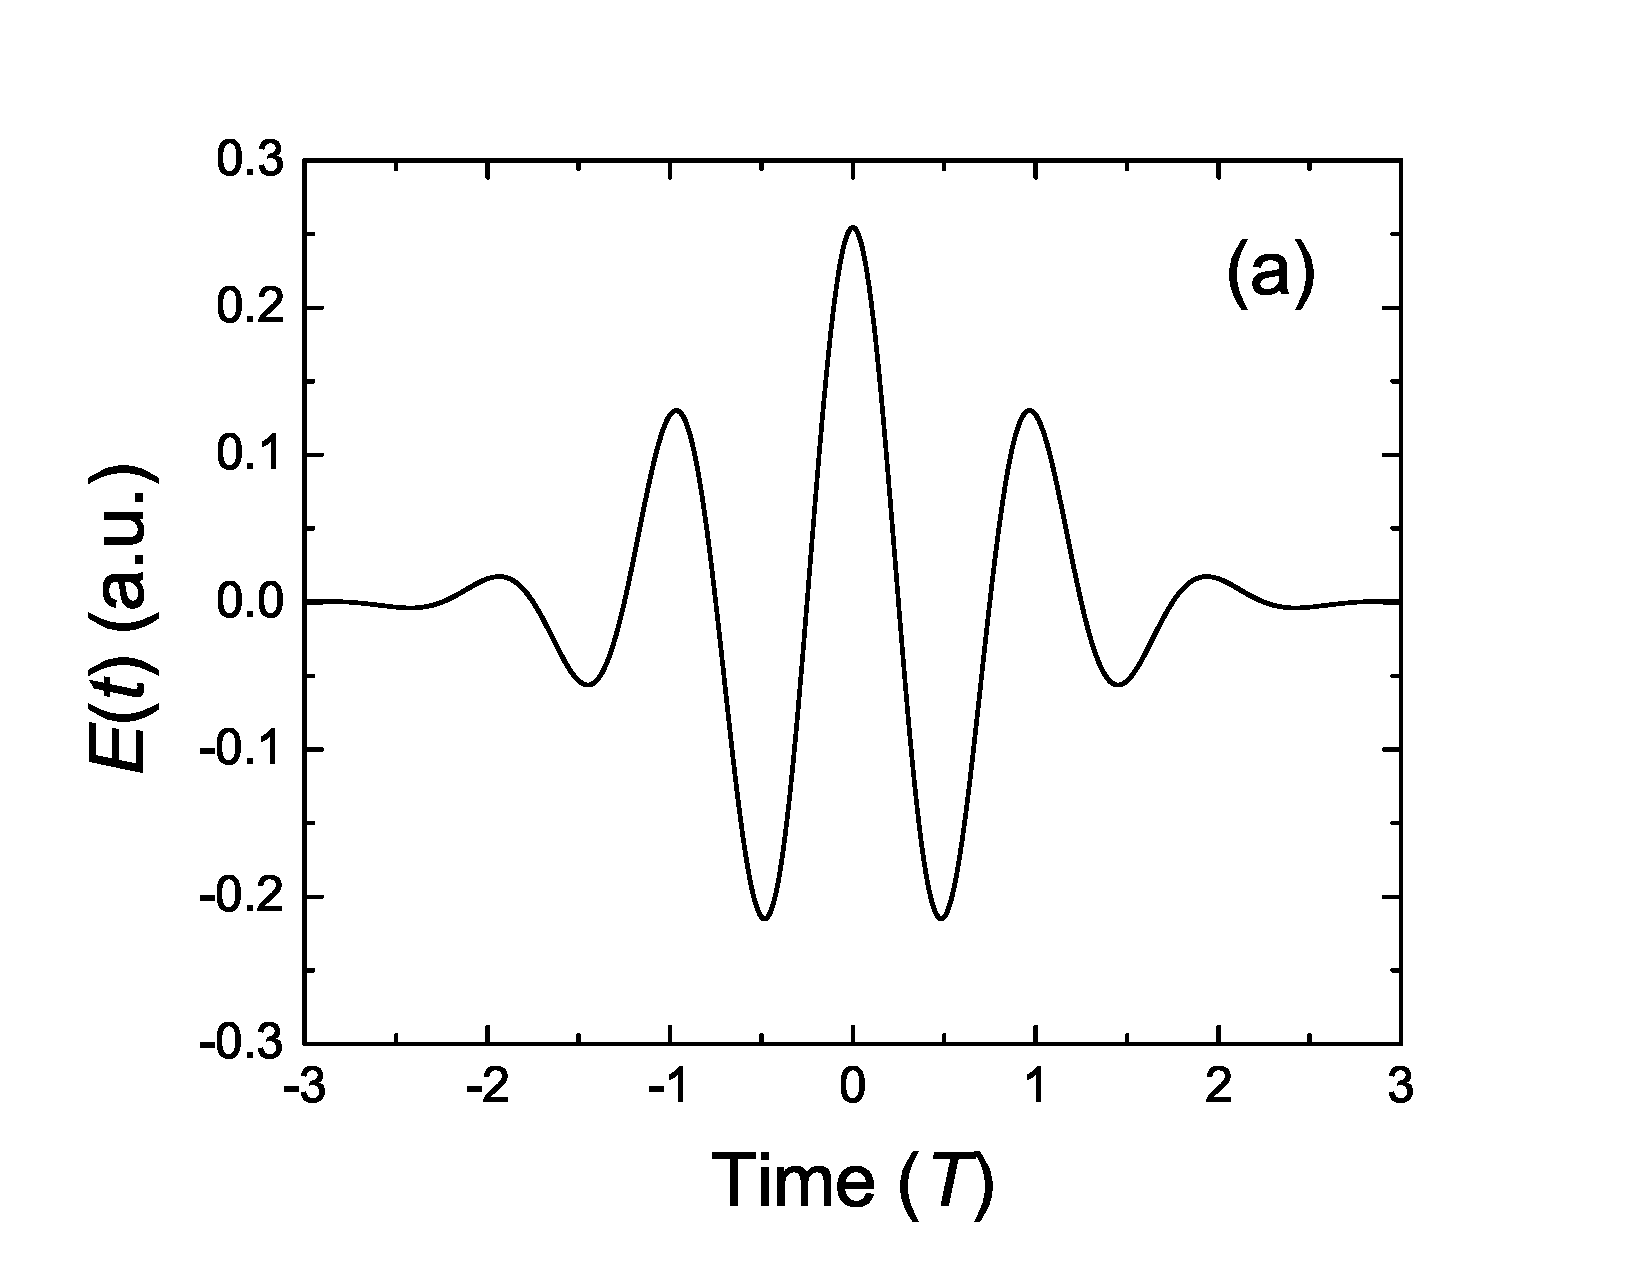
\includegraphics[width=0.27\textwidth,height=0.2\textwidth]{fig1a.eps}
	}
	\hspace{0.1in}
	\subfigure{
		\label{fig1b}
		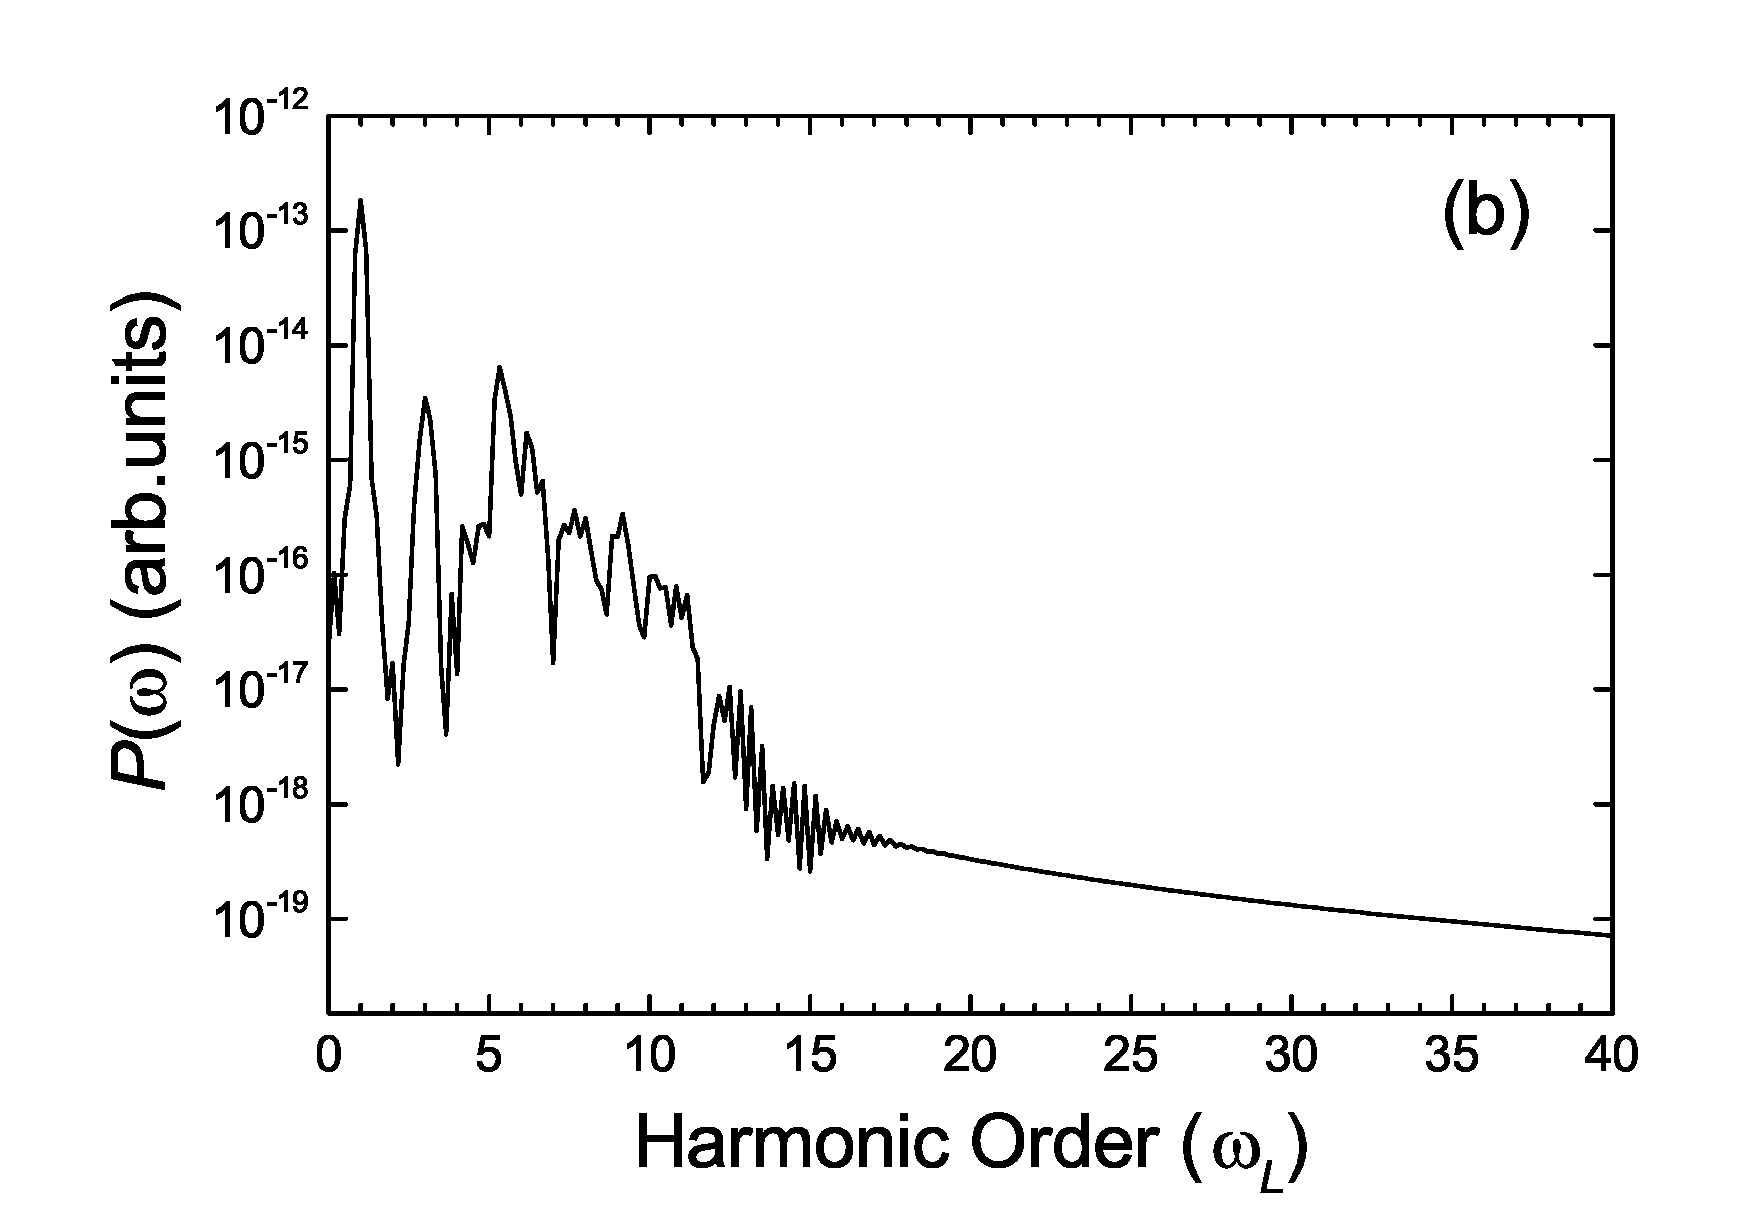
\includegraphics[width=0.27\textwidth,height=0.2\textwidth]{fig1b.eps}
	}
	\hspace{0.1in}
	\subfigure{
		\label{fig1c}
		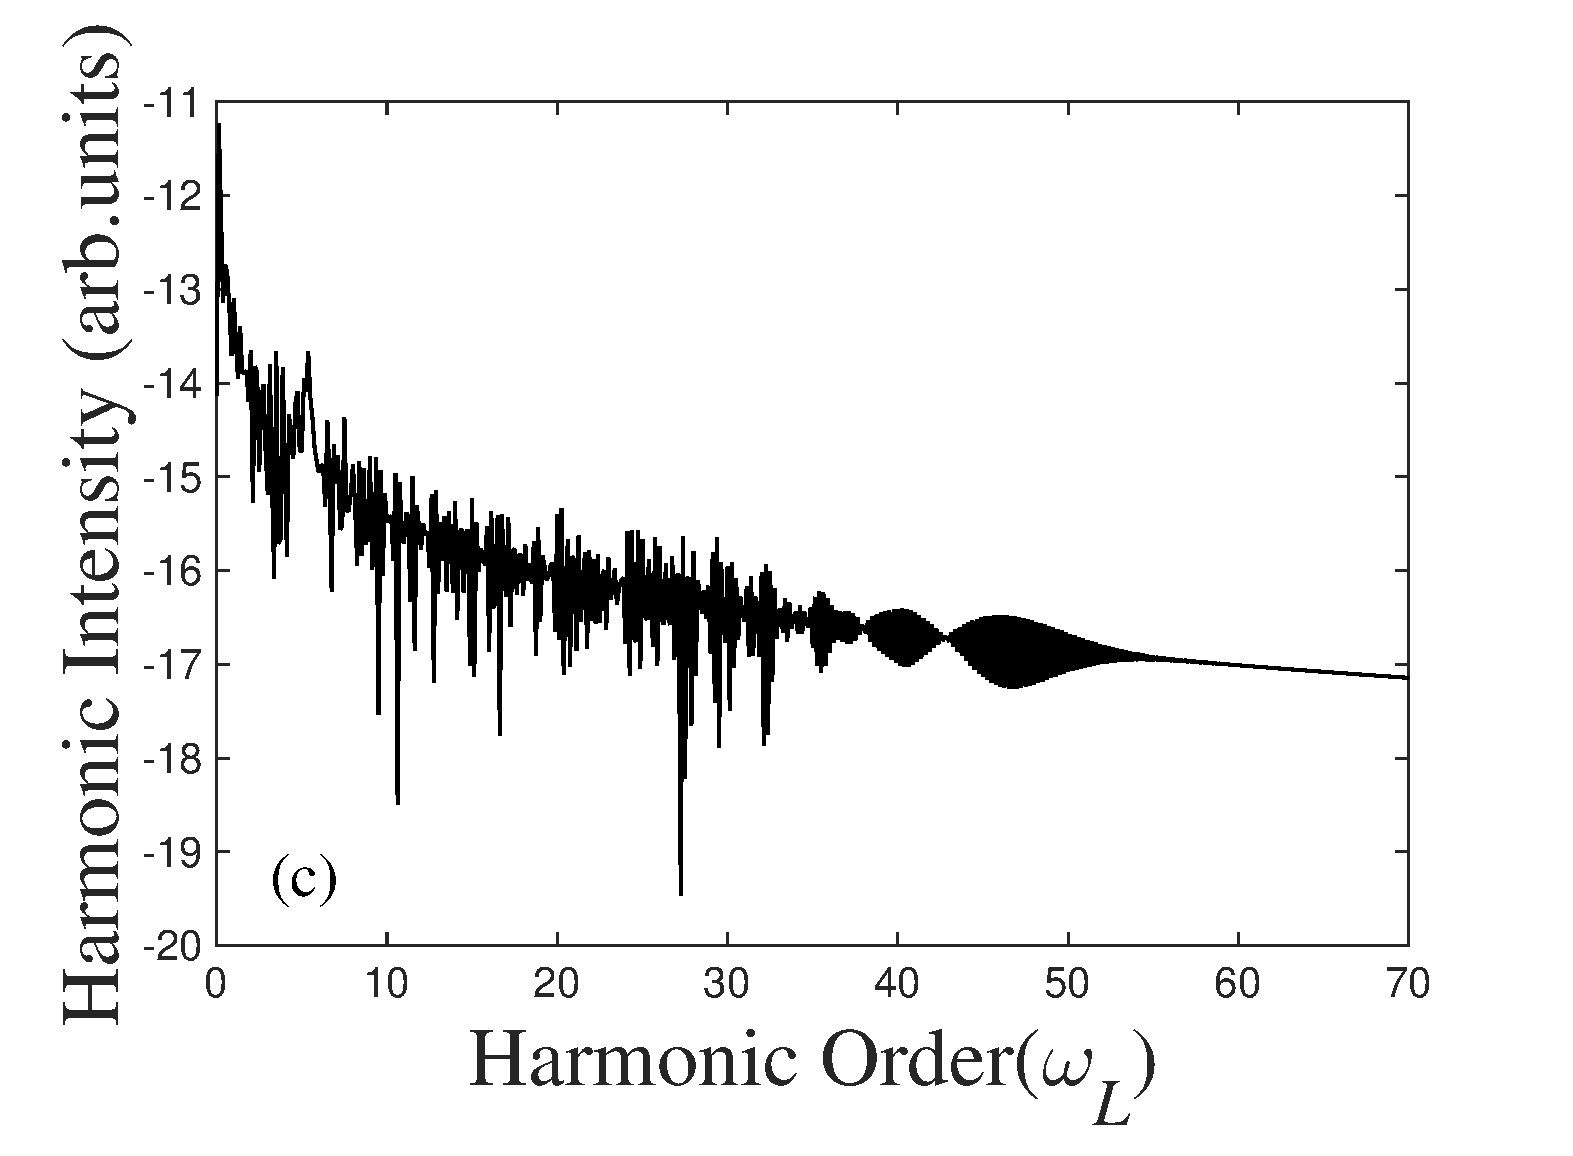
\includegraphics[width=0.27\textwidth,height=0.2\textwidth]{fig1c.eps}
	}
	
	\subfigure{
		\label{fig1d}
		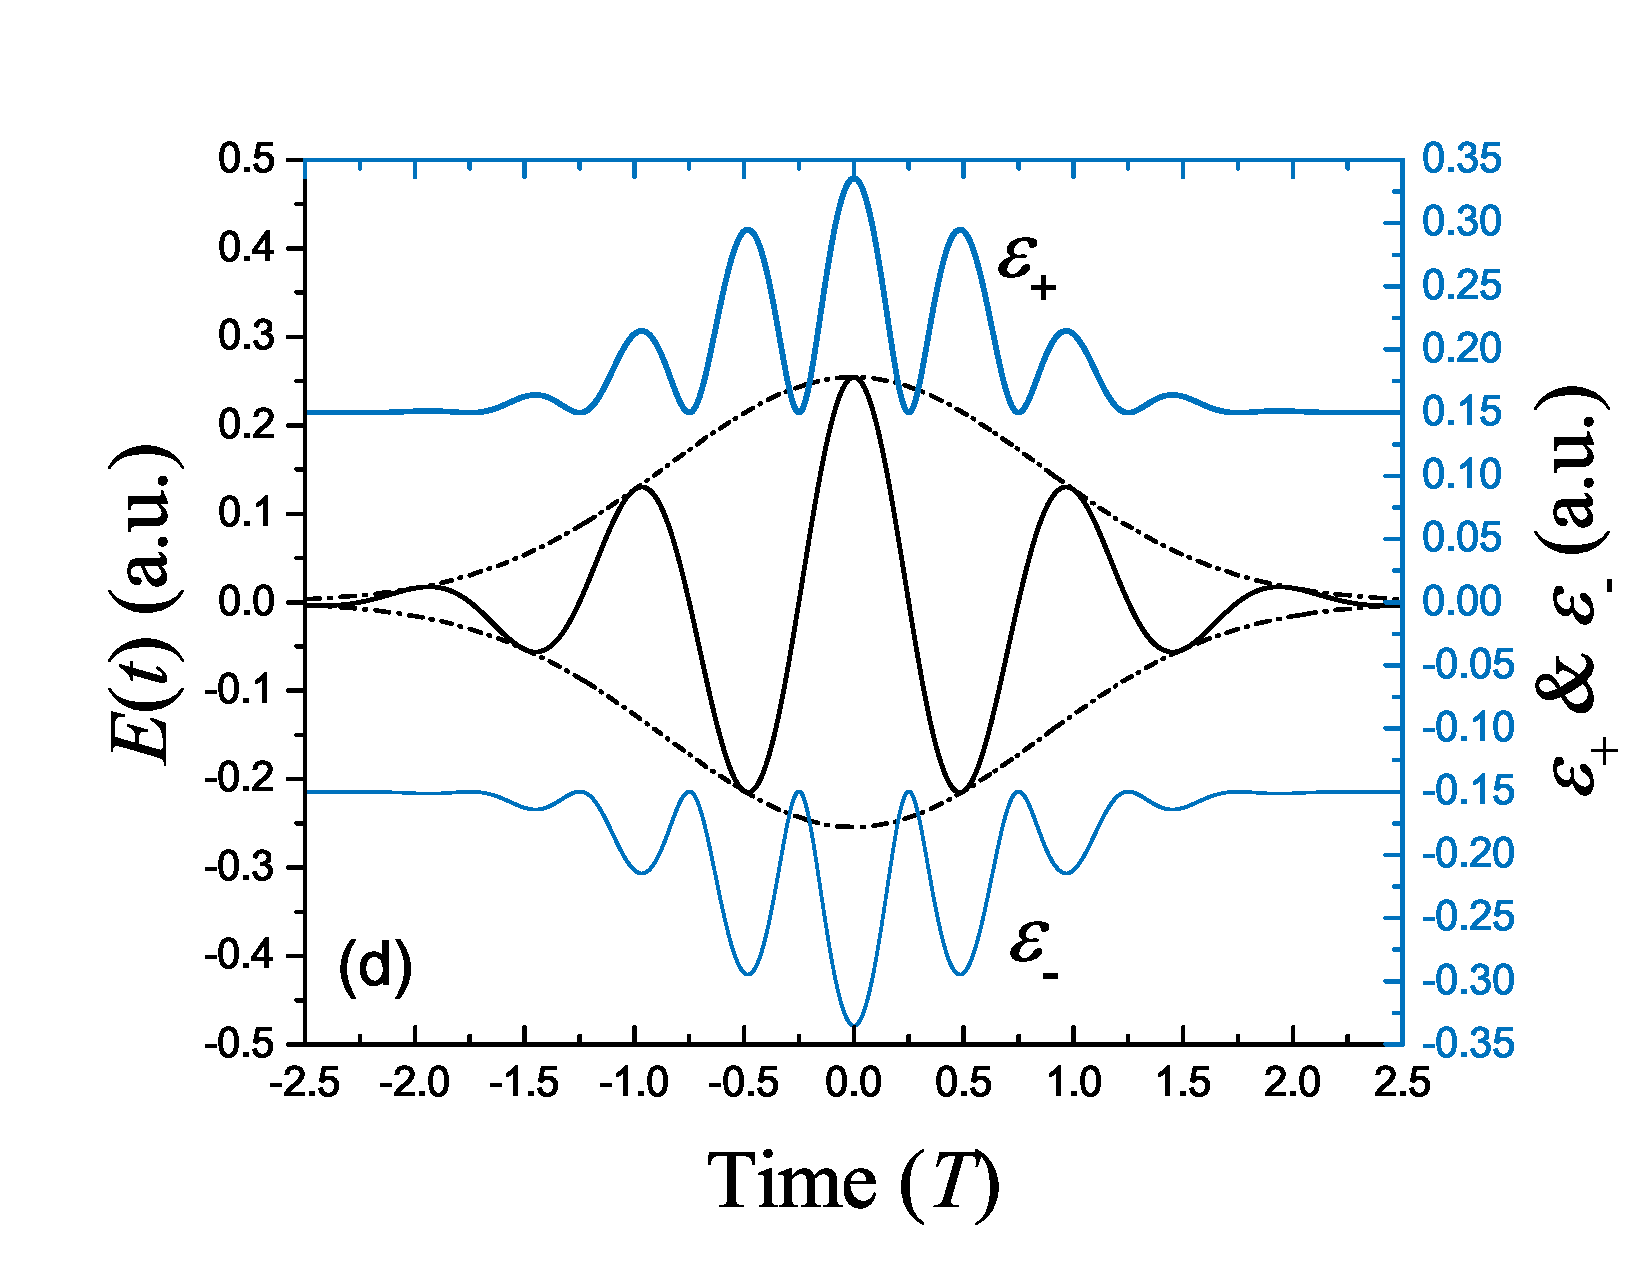
\includegraphics[width=0.3\textwidth,height=0.2\textwidth]{fig1d.eps}
	}
	\subfigure{
		\label{fig1e}
		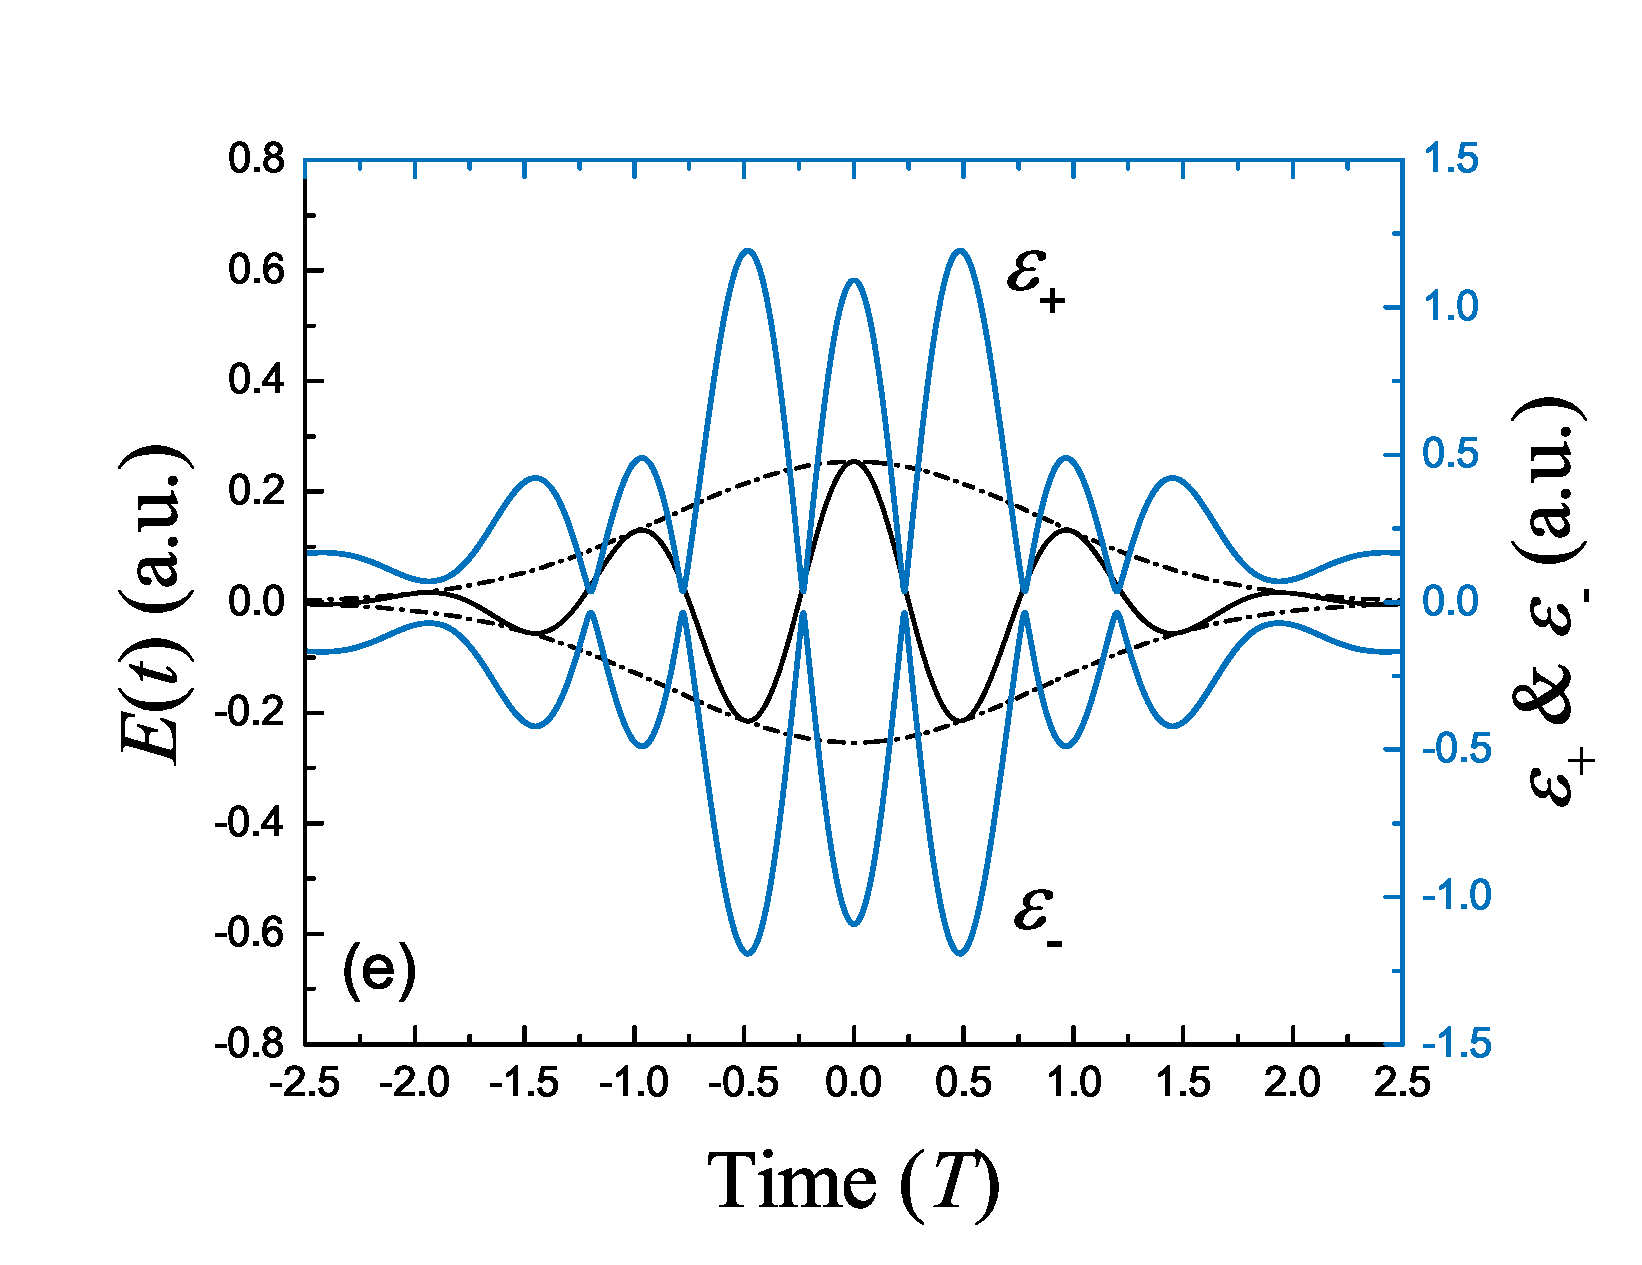
\includegraphics[width=0.3\textwidth,height=0.2\textwidth]{fig1e.eps}
	}
	\subfigure{
		\label{fig1f}
		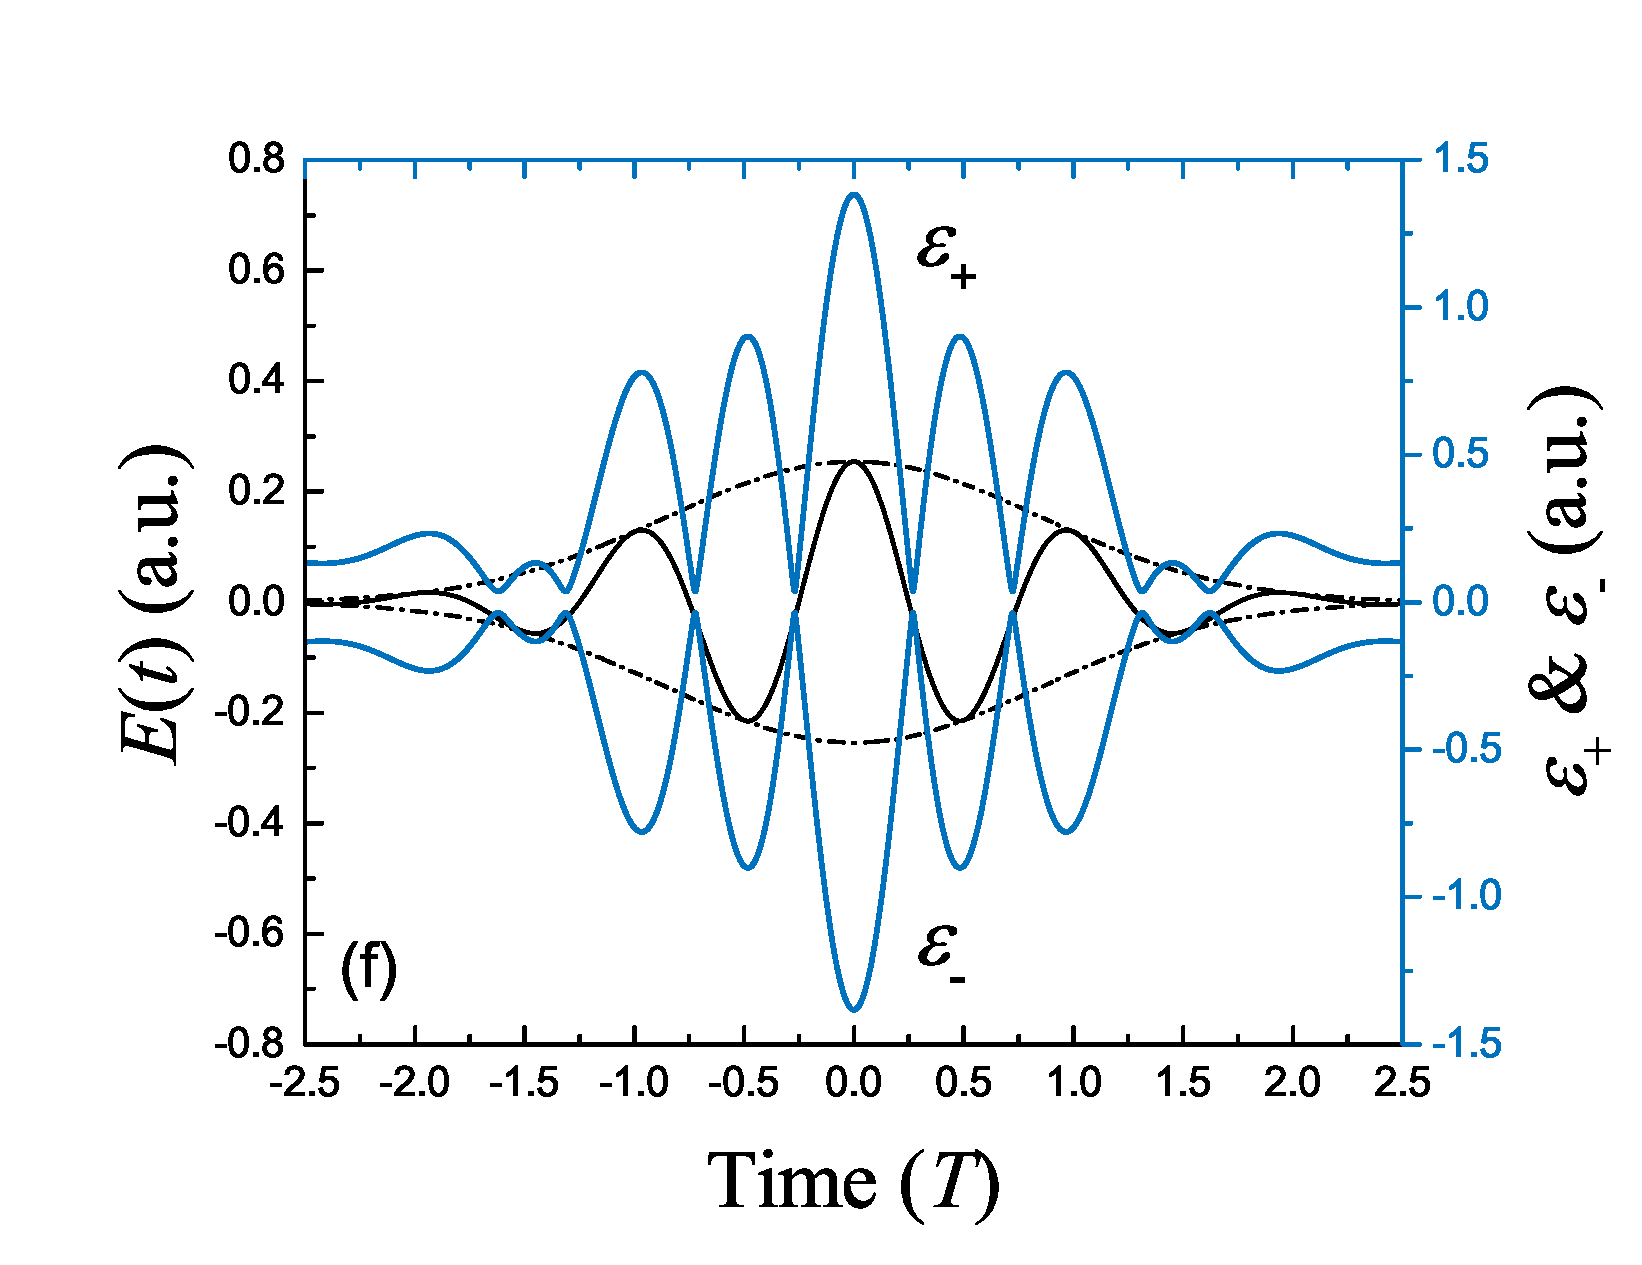
\includegraphics[width=0.3\textwidth,height=0.2\textwidth]{fig1f.eps}
	}
	\subfigure{
		\label{fig1g}
		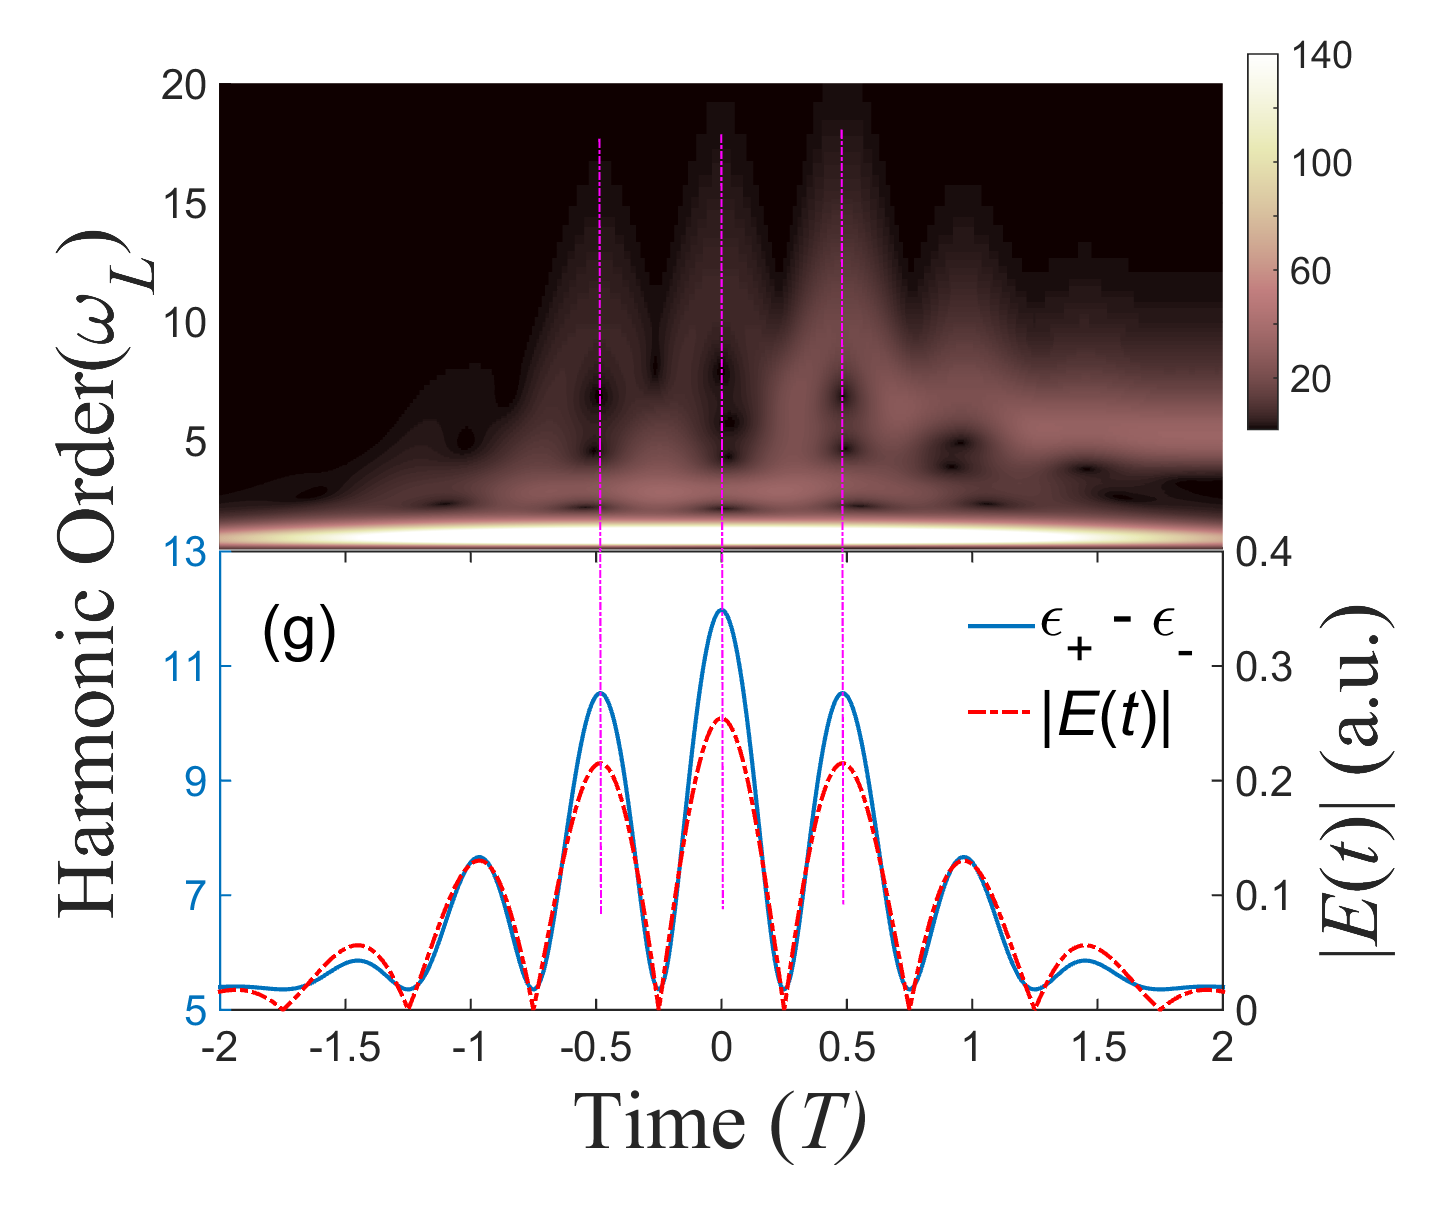
\includegraphics[width=0.3\textwidth,height=0.2\textwidth]{fig1g.eps}
	}
	\subfigure{
		\label{fig1h}
		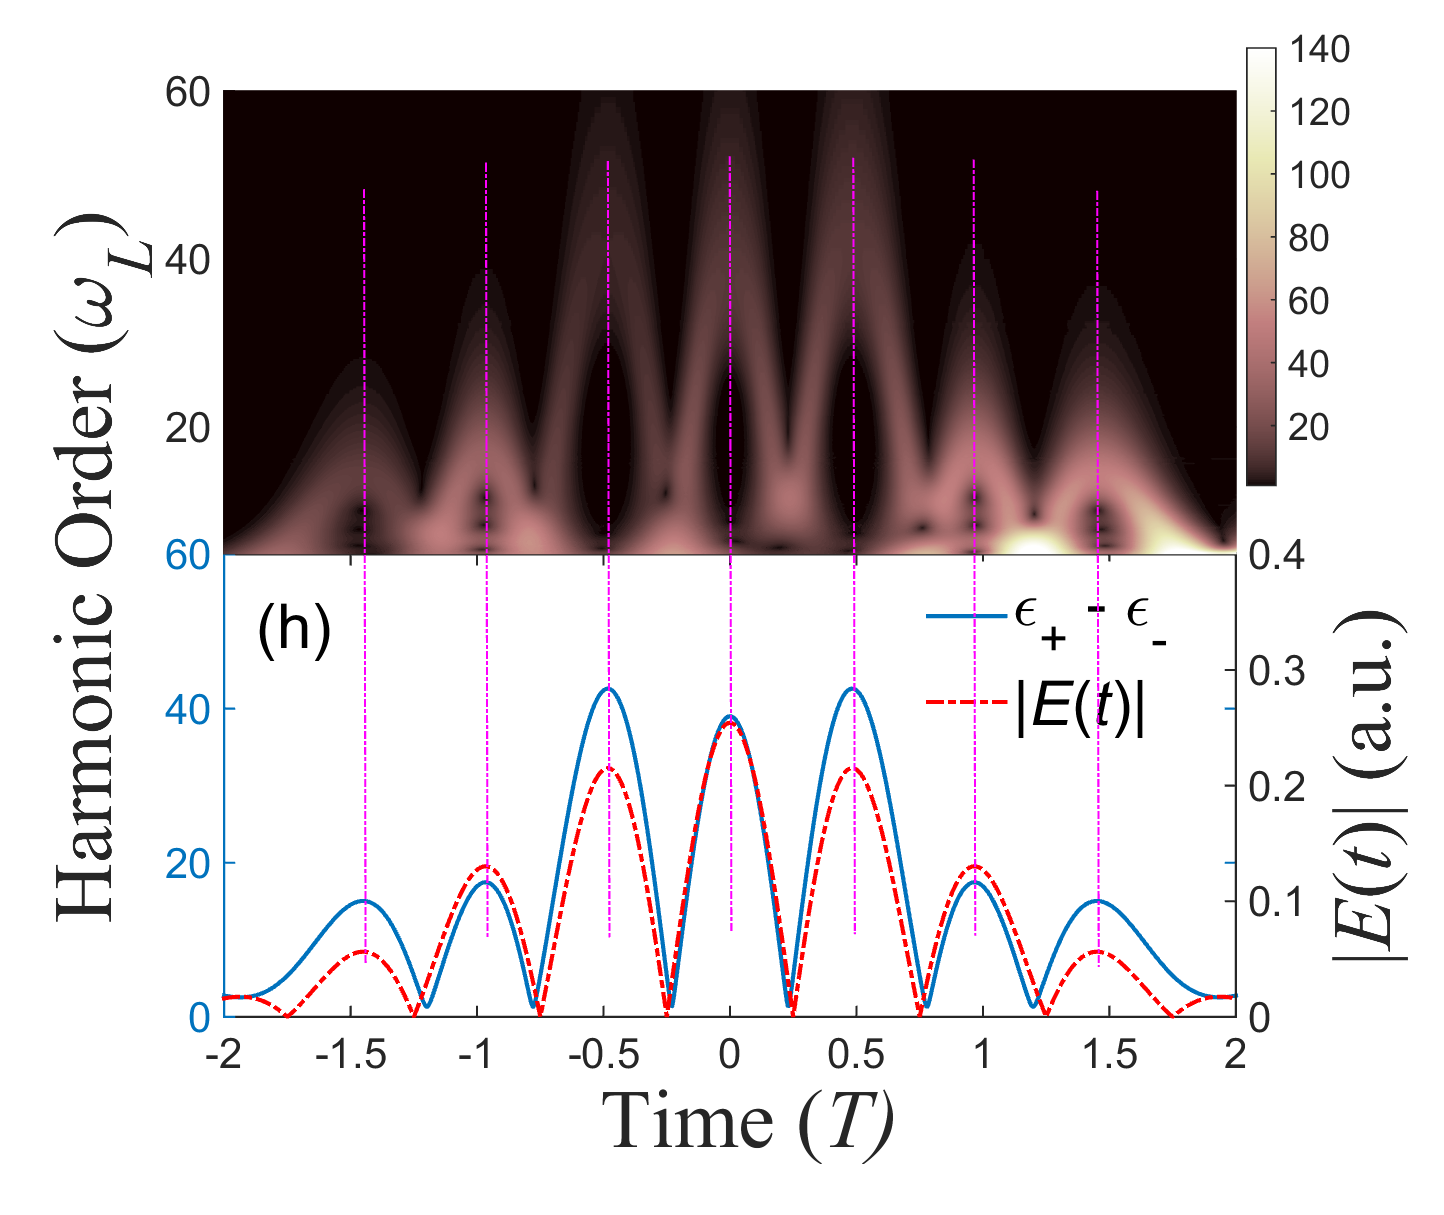
\includegraphics[width=0.3\textwidth,height=0.2\textwidth]{fig1h.eps}
	}
	\subfigure{
		\label{fig1i}
		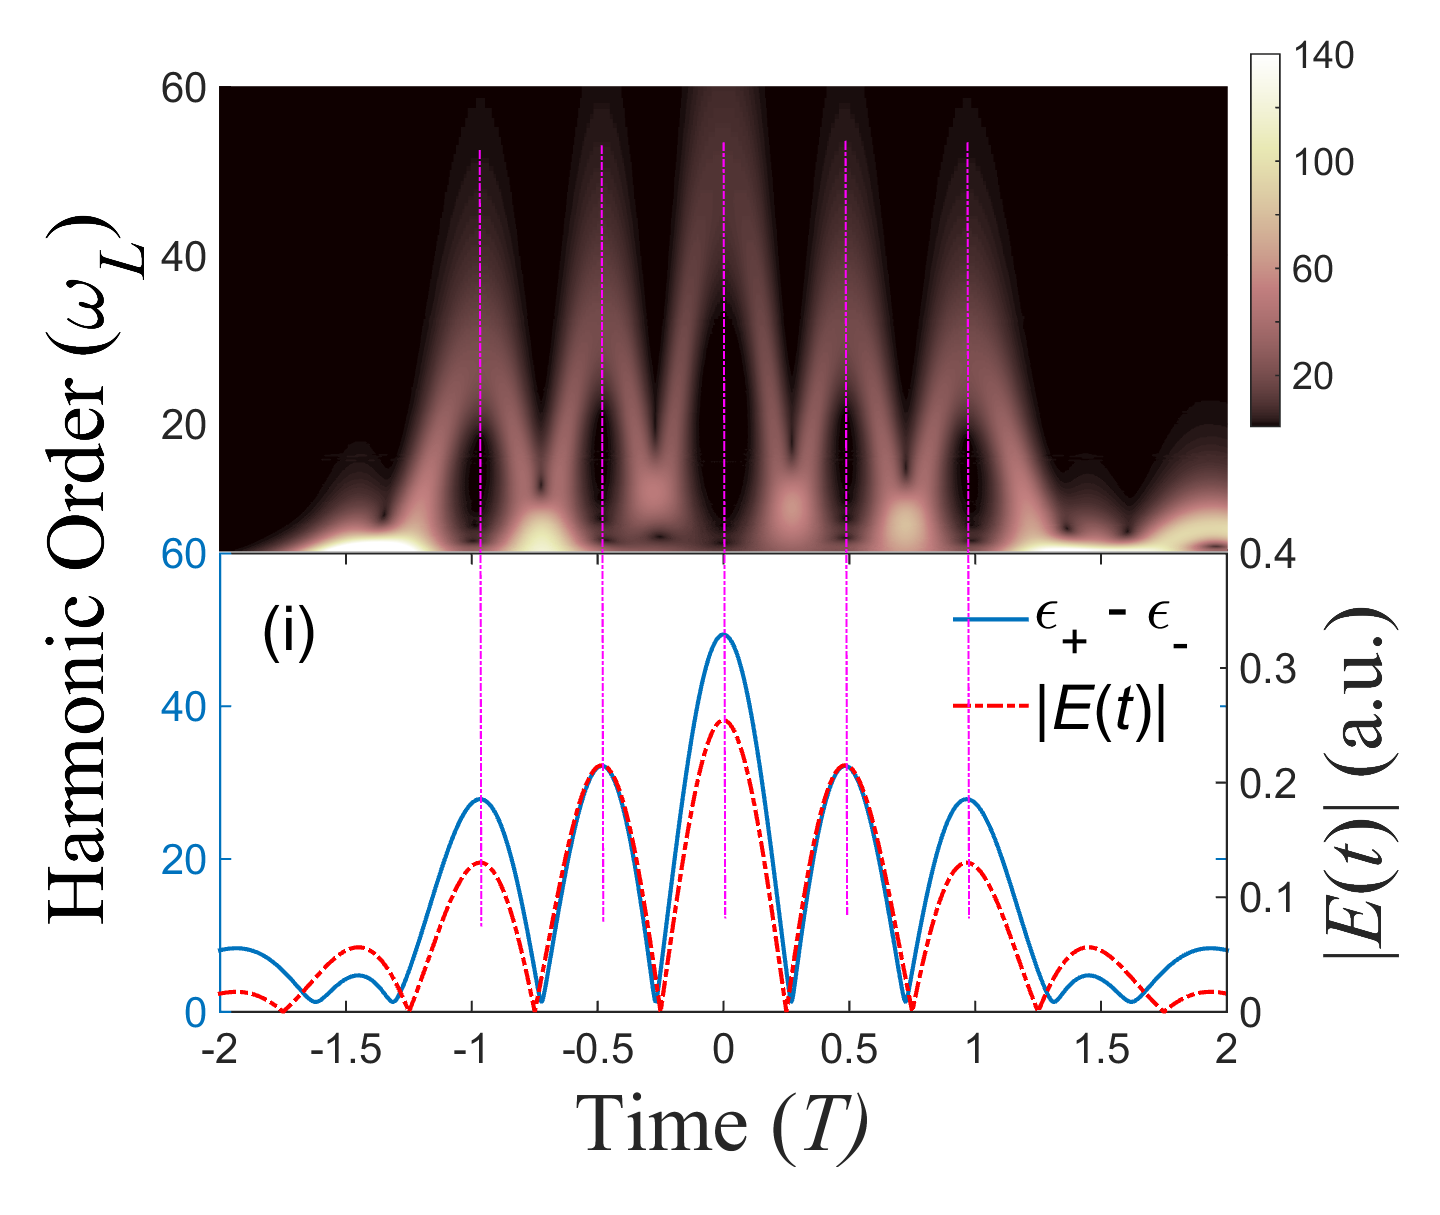
\includegraphics[width=0.3\textwidth,height=0.2\textwidth]{fig1i.eps}
	}
	\caption{HHG analysis for three permanent dipole moments, $\mu_{11}=\mu_{22}=0(\xi=0)$ [the left column], $\mu_{11}=-\mu_{22}=-4\mu_{21} (\xi=4)$ [the middle column], and $\mu_{11}=-\mu_{22}=4\mu_{21}$ [the right column]. The uppermost row show the HHG spectra; the middle row show the time-dependent eigenvalues of the two dressed states $\epsilon_{+}$ and $\epsilon_{-}$; and the lowest row show the time-frequency spectra, while the lower panel shows the time-dependent energy separation between the two dressed states $\epsilon_{+}-\epsilon_{-}$ (the harmonic energy predicted by two-level model) and the laser pulse absolute amplitude. Parameters for this laser pulse are: central frequency $\omega_L=0.056\;\text{a.u.}$, duration $\tau=5.43\;\text{fs}$, and peak Rabi frequency $\Omega_0=0.30\;\text{a.u.}$.}
	\label{fig1}
\end{figure} 

Besides, comparing the right two columns, it is found that the harmonic generation process is also sensitive to the property of permanent dipole moment: for negative $\xi$ (the right column), the cutoff harmonic is emitted only at laser pulse peak time, while for positive $\xi$ (the middle column), it is emitted at both sides of the peak with about $0.5T$ interval to the peak time. As we know that, this phenomenon has not been mentioned before. But it is easy understood using formula (\ref{eq14}): according to the mathematical theory, for different given $\xi$, $\omega_{\rm{max}}$ may occur at different time point. In addition, as shown in the lower panels of the lowest row figures, the time-frequency HHG spectrum shares the same temporal shape with the laser pulse absolute amplitude \cite{CuiNi2010NJP-wavelet}. Even though there's little difference existing for the case of positive $\xi$, but at least the minimum time and peak time of the time-frequency spectrum are totally same with those of the laser pulse absolute amplitude as the vertical dashed lines shown. 
    
\subsubsection{introduce of the chirp}
Note that, as shown in Figs. \ref{fig1h} and \ref{fig1i}, even though the harmonic cutoff energy can be largely extended, the HHG spectra exhibit more than five well-formed individual peak structures in the plateau region, which means that the plateau harmonics have more than ten quantum trajectories (five long trajectories and five short trajectories). If one select these plateau harmonics to synthesize an attosecond pulse, there would be a APT with ten individual peaks generated. However, people have been dedicated to obtain an IAP with short duration for many years \cite{IAP-reference1-1998,Sansone-Polarization-gate-Nature-2006,IAP-reference2-2008,IAP-reference3-2008,IAP-reference4-2012}. If there's a method which can reduce the plateau harmonic's quantum trajectory number, an APT with less peaks or even an IAP may be generated. As we know that the laser pulse can be shaped by introducing the chirped frequency. Since the time-frequency HHG spectrum shares the same shape with the laser pulse absolute amplitude, we expect the chirp introducing could reduce the quantum trajectory number. 

The chirp chosen is with a hyperbolic tangent form, and the time-dependent carrier envelope phase $ \varphi(t) $ in Eq. (\ref{eq3}) is then written as:

\begin{equation}
\varphi \left( t \right) =  - \eta \tanh \left[ {{{\left( {t - {t_d}} \right)} \mathord{\left/
			{\vphantom {{\left( {t - {t_d}} \right)} {{\tau _c}}}} \right.
			\kern-\nulldelimiterspace} {{\tau _c}}}} \right].
\label{eq15}
\end{equation}
Where $ \tau_{\rm{c}} $ is the steepness of the chirp function and $ t_{\rm{d}} $ is set at the middle of the sweep here. $ \eta $  denotes the frequency sweeping range. If $ \eta=0 $, driving pulse is chirp free. This is chirp form has been used by many other researchers \cite{Carrera-Chirp-PRA-2007,CuiNi2010NJP-wavelet,Chirp-Reference-2013PRA}.

With a chirp, as shown in Fig. \ref{fig2a}, the laser pulse's temporal shape changes significantly to that without chirp, and its origin oscillatory periodicity and up-down symmetry disappear: the central part of the carrier wave gets broader, the side parts become weaker, while the peak amplitude is remained. Importantly, the introduce of chirp makes the absolute amplitude difference between the pulse central peak and its neighbored ones get larger. According to the rapid level crossing theory, the time-frequency HHG spectrum shares the same shape with the laser pulse absolute amplitude \cite{CuiNi2010NJP-wavelet}. Therefore, if the permanent dipole moment is $\mu_{11}=-\mu_{22}=4\mu_{21}(\xi=-4)$ as the right column in Fig. \ref{fig1}, it's easy to speculate that the HHG spectrum would have a large plateau whose harmonics have only two quantum trajectories at most. This trajectory number is much less than that of the case without chirp. Thus, an APT with only two peaks can be synthesized using these plateau harmonics. However, it can be seen from Fig. \ref{fig2a} that, the introduce of chirp has weakened steepness of the laser pulse peak's rising and falling edges which results from the getting broader of the center carrier. As mentioned before, the time-frequency HHG spectrum shares the same shape with the laser pulse absolute amplitude. Therefore, this steepness weakening may lead to the enlargement of atto-chirp \cite{attochirp-ref1-2003,attochirp-ref2-2007,attochirp-ref3-2009} for both long and short quantum trajectories, and this can increase the duration for both peaks of generated APT. However, it is contradictory for the center carrier to get narrower and for the absolute amplitude difference between the pulse central peak and its neighbored ones to get larger. Thus, a proper group of chirp parameters are chosen here as $\eta=6.25,\;\tau_{\rm{c}}=120$, which can make the absolute amplitude difference quite large and the center carrier not too broad, as shown in Fig. \ref{fig2a}.

\begin{figure}[!htbp]
	\centering
	\subfigure{
		\label{fig2a}
		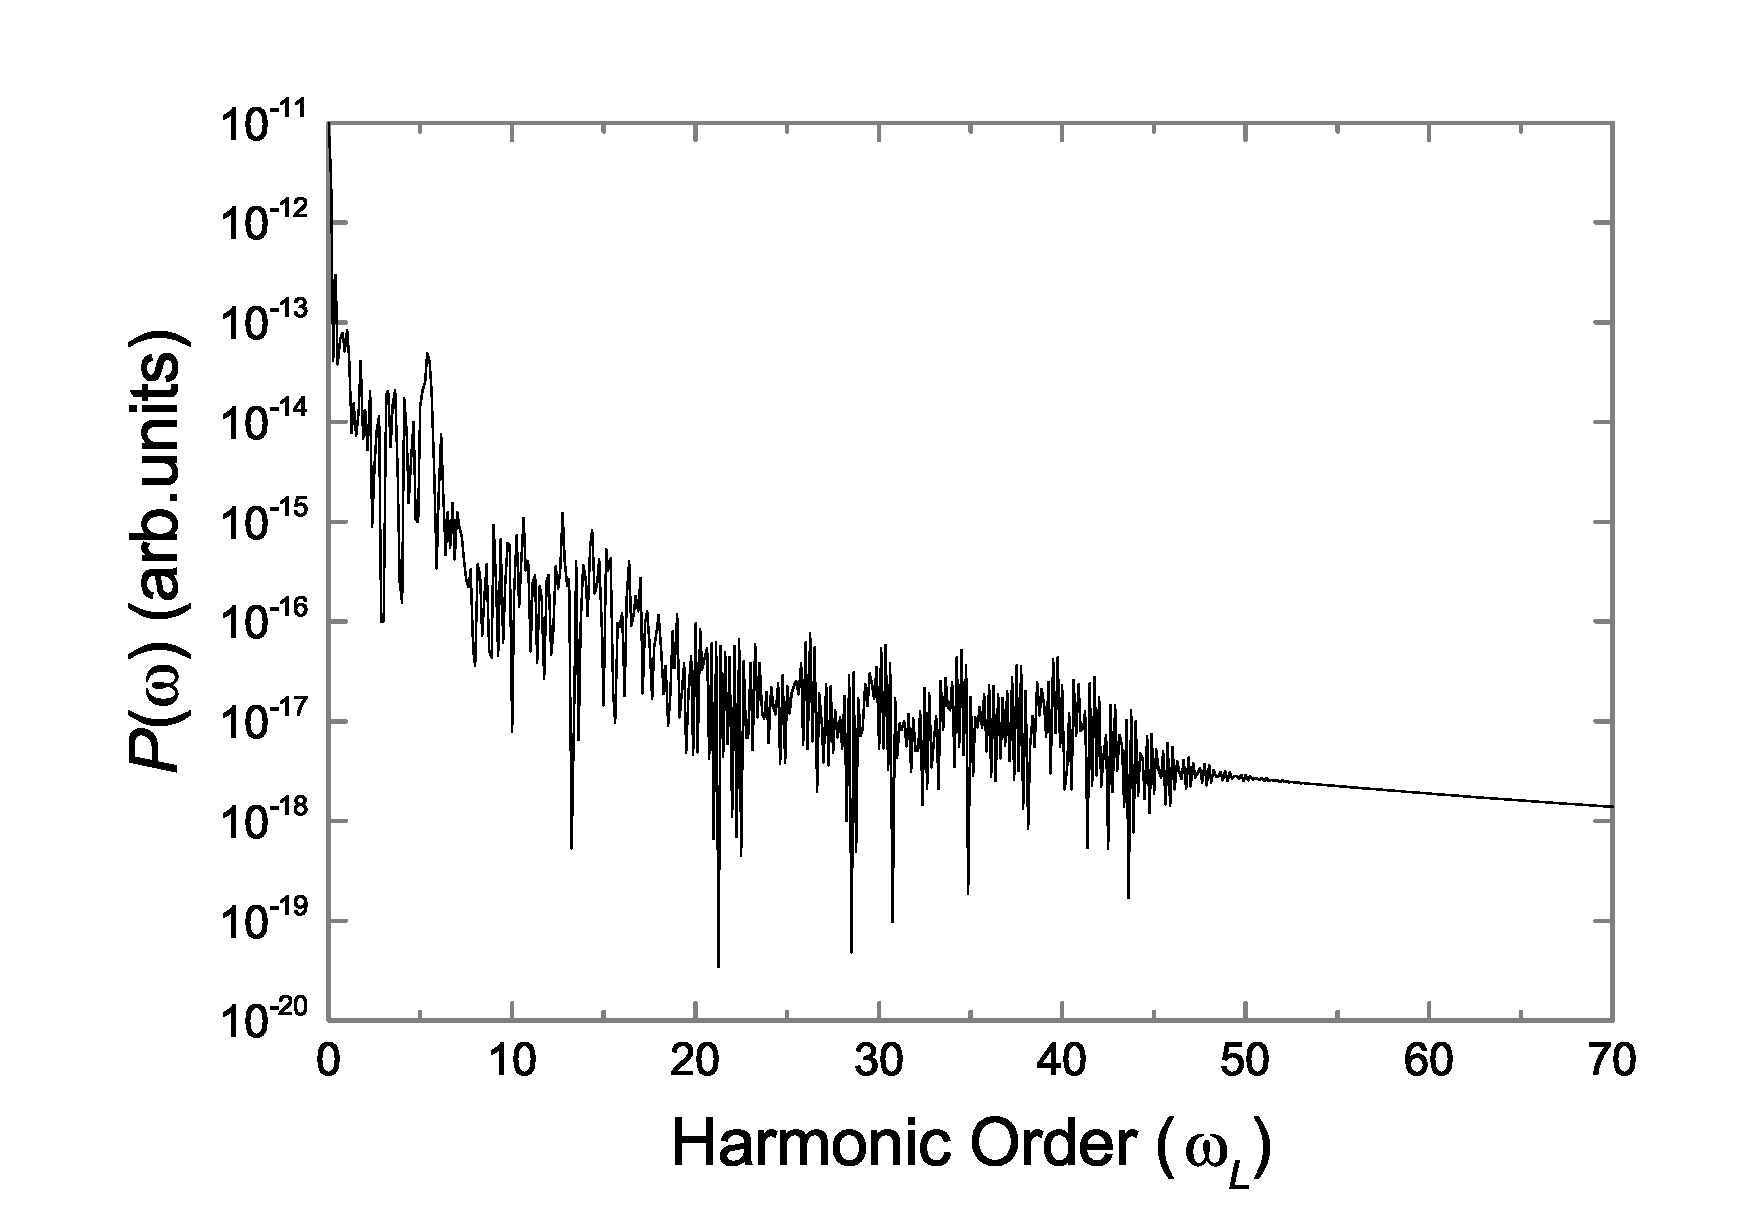
\includegraphics[width=0.30\textwidth]{fig2a.eps}
	}
	\subfigure{
		\label{fig2b}
		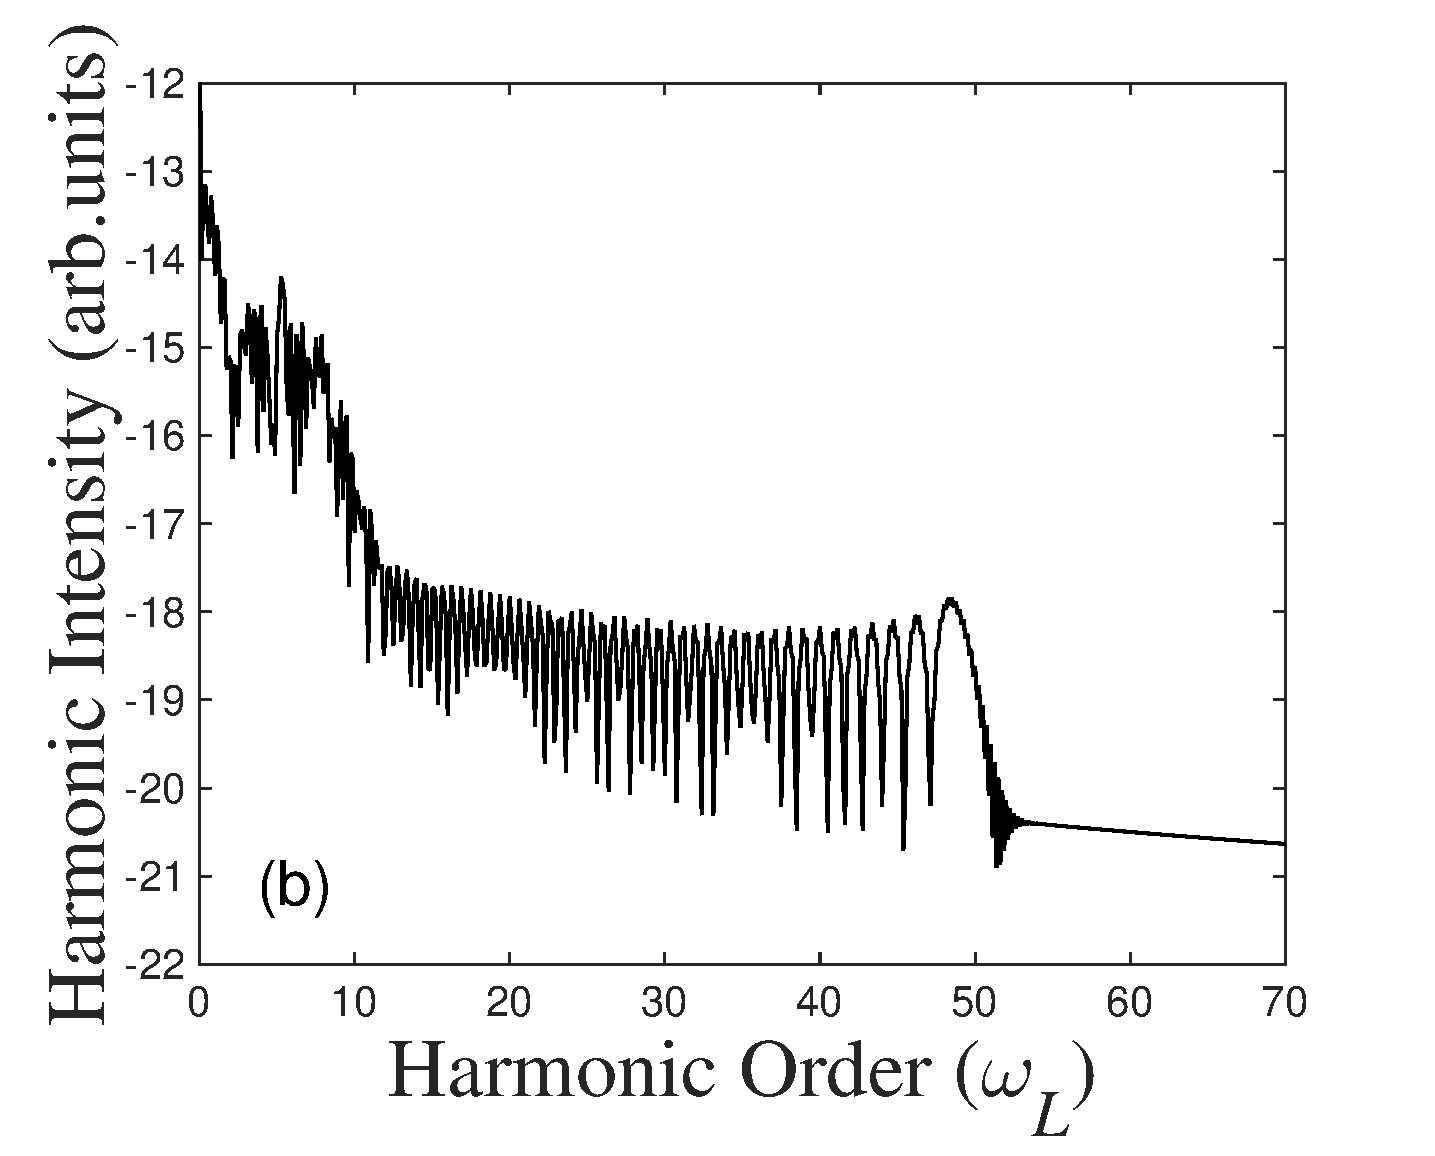
\includegraphics[width=0.30\textwidth]{fig2b.eps}
	}
	\subfigure{
		\label{fig2c}
		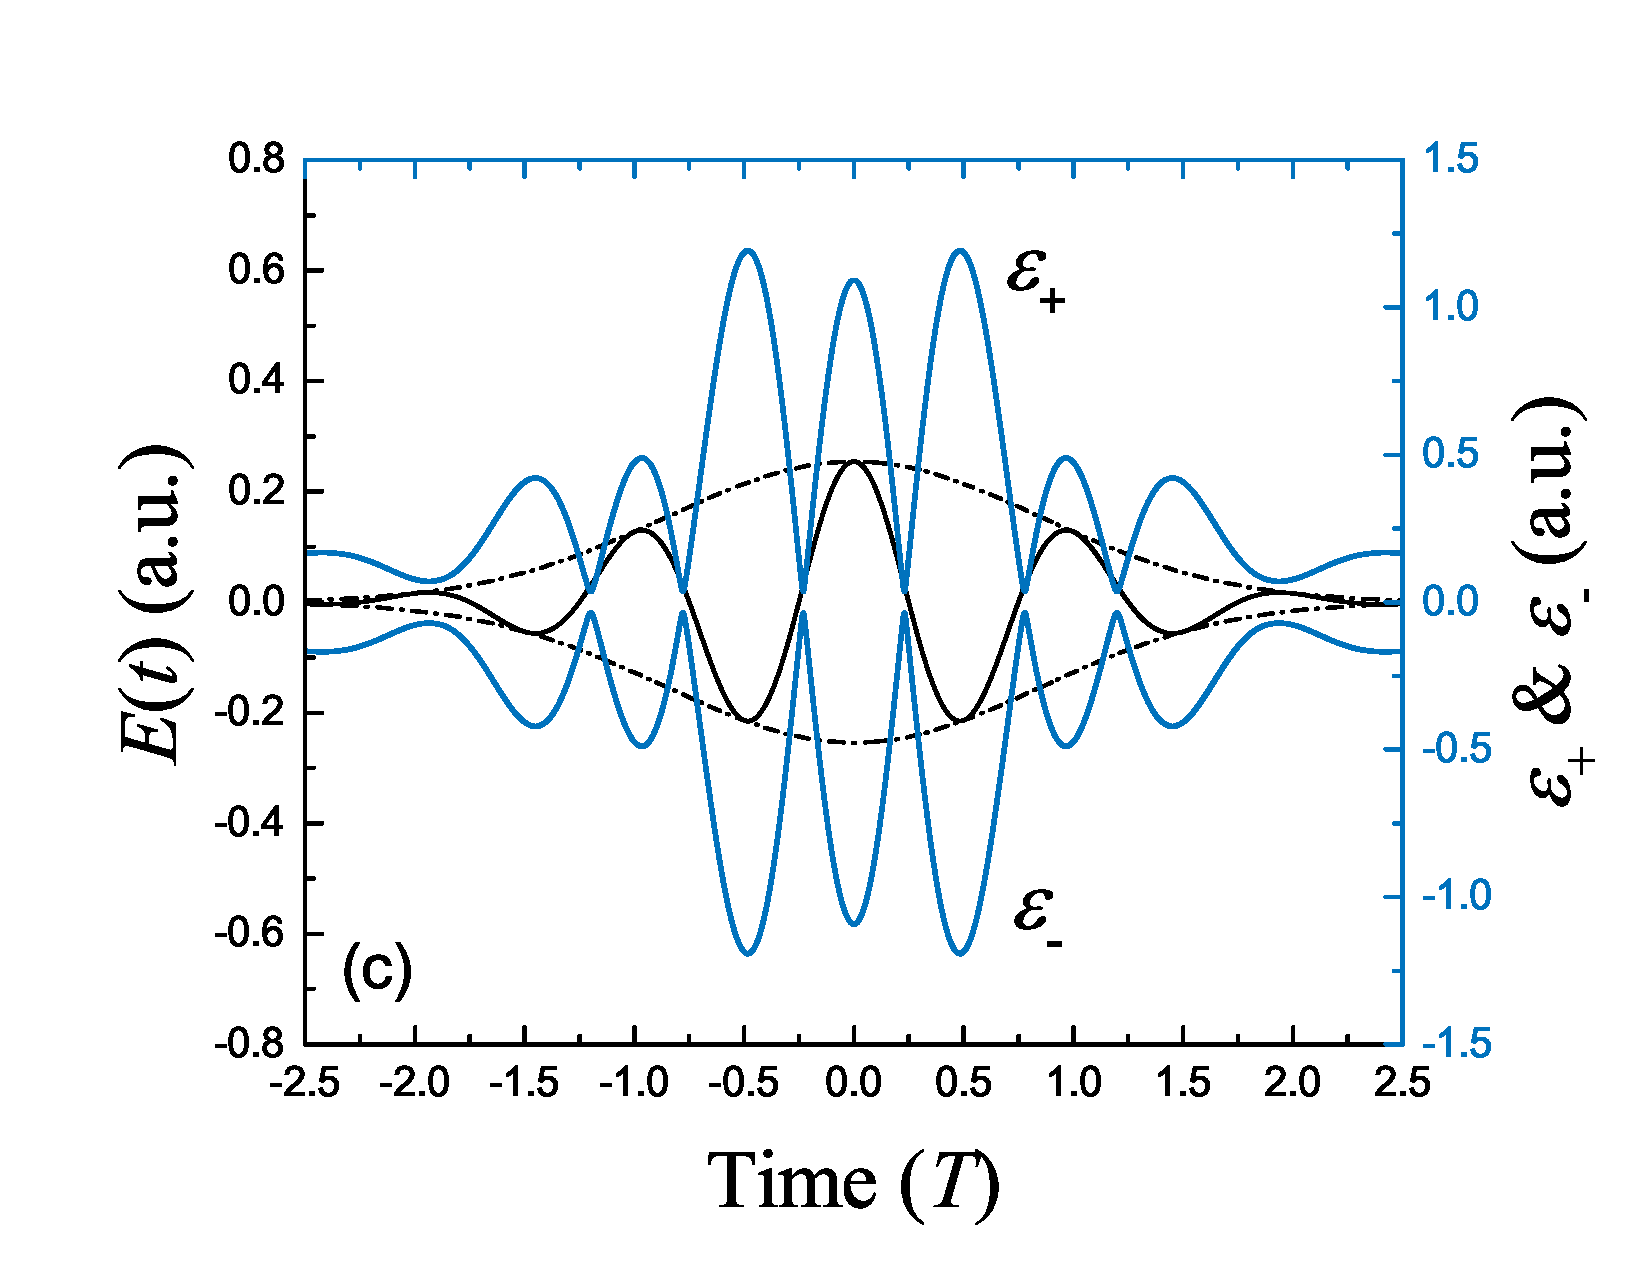
\includegraphics[width=0.30\textwidth]{fig2c.eps}
	}
	\caption{(a) The laser pulse with and without chirped frequency, (b) the corresponding HHG spectrum from the driven-two-level polar medium [$\mu_{11}=4,\;\mu_{22}=-4(\xi=-4)$], and (c) the wavelet time-frequency analysis. The lower panel of figure (c) shows time-dependent energy separation between the two dressed states $\epsilon_{+}-\epsilon_{-}$ (the harmonic energy predicted by two-level model) and the absolute amplitude of laser field as in Figs. \ref{fig1g}, \ref{fig1h} and \ref{fig1i}. The chirp parameters are: $\eta=6.25$, $\tau_c=120$. The other laser and two-level polar medium parameters are same with those in Fig. \ref{fig1}.}
	\label{fig2}
\end{figure}

Fig. \ref{fig2b} shows the corresponding HHG spectrum of the two-level polar medium [$\mu_{11}=-\mu_{22}=4\mu_{21}(\xi=-4)$]. Its time-frequency profile is shown in Fig. \ref{fig2c}. With the same permanent dipole moment, the cutoff harmonic should emit at laser pulse peak time as shown in Fig. \ref{fig1i}. Therefore, according to Eq. \ref{eq14}, the harmonic spectra should have the same cutoff energy with the non-chirp case. This is confirmed by the numerical simulation results in Figs. \ref{fig2b} and \ref{fig2c}. There are only two well-formed individual peak structures besides the central peak in the time-frequency spectrum while the case without chirp has four ones. Moreover, these peak values are much smaller than those of case without chirp, this makes the value difference between the central peak and the sub-peak much larger than that of non-chirp case shown in Fig. \ref{fig1i}. Therefore, within a large plateau region, the harmonics would have two quantum trajectories. One can use harmonics within this region to synthesize an APT with only two individual peaks.  

Consequently, we will use the plateau harmonics to synthesize attosecond pulses inorder to verify our conjecture. Both cases with and without chirp are investigated for comparison. All the harmonics (including the even orders) from 14th to 29th are selected for both cases. The results are shown in Fig. \ref{fig3}. Every duration value of all peaks is marked in the figures. There is an APT generated with ten individual peaks for the case without chirp, while there is an APT generated which has only two individual peaks (we call it attosecond pulse pair, APP). This is completely consistent with the quantum trajectory numbers in the plateau region (shown in Figs. \ref{fig1i} and \ref{fig2c}). Therefore, we have successfully reduced the individual peak numbers of the generated APT by introducing chirp frequency to the driving laser pulse. However, there is no an IAP generated. In addition, as shown in Fig. \ref{fig3b}, the increase of durations for both two center peaks confirms that the chirp frequency could enlarge the atto-chirp.

\begin{figure}[!htbp]
	\centering
	\subfigure{
		\label{fig3a}
		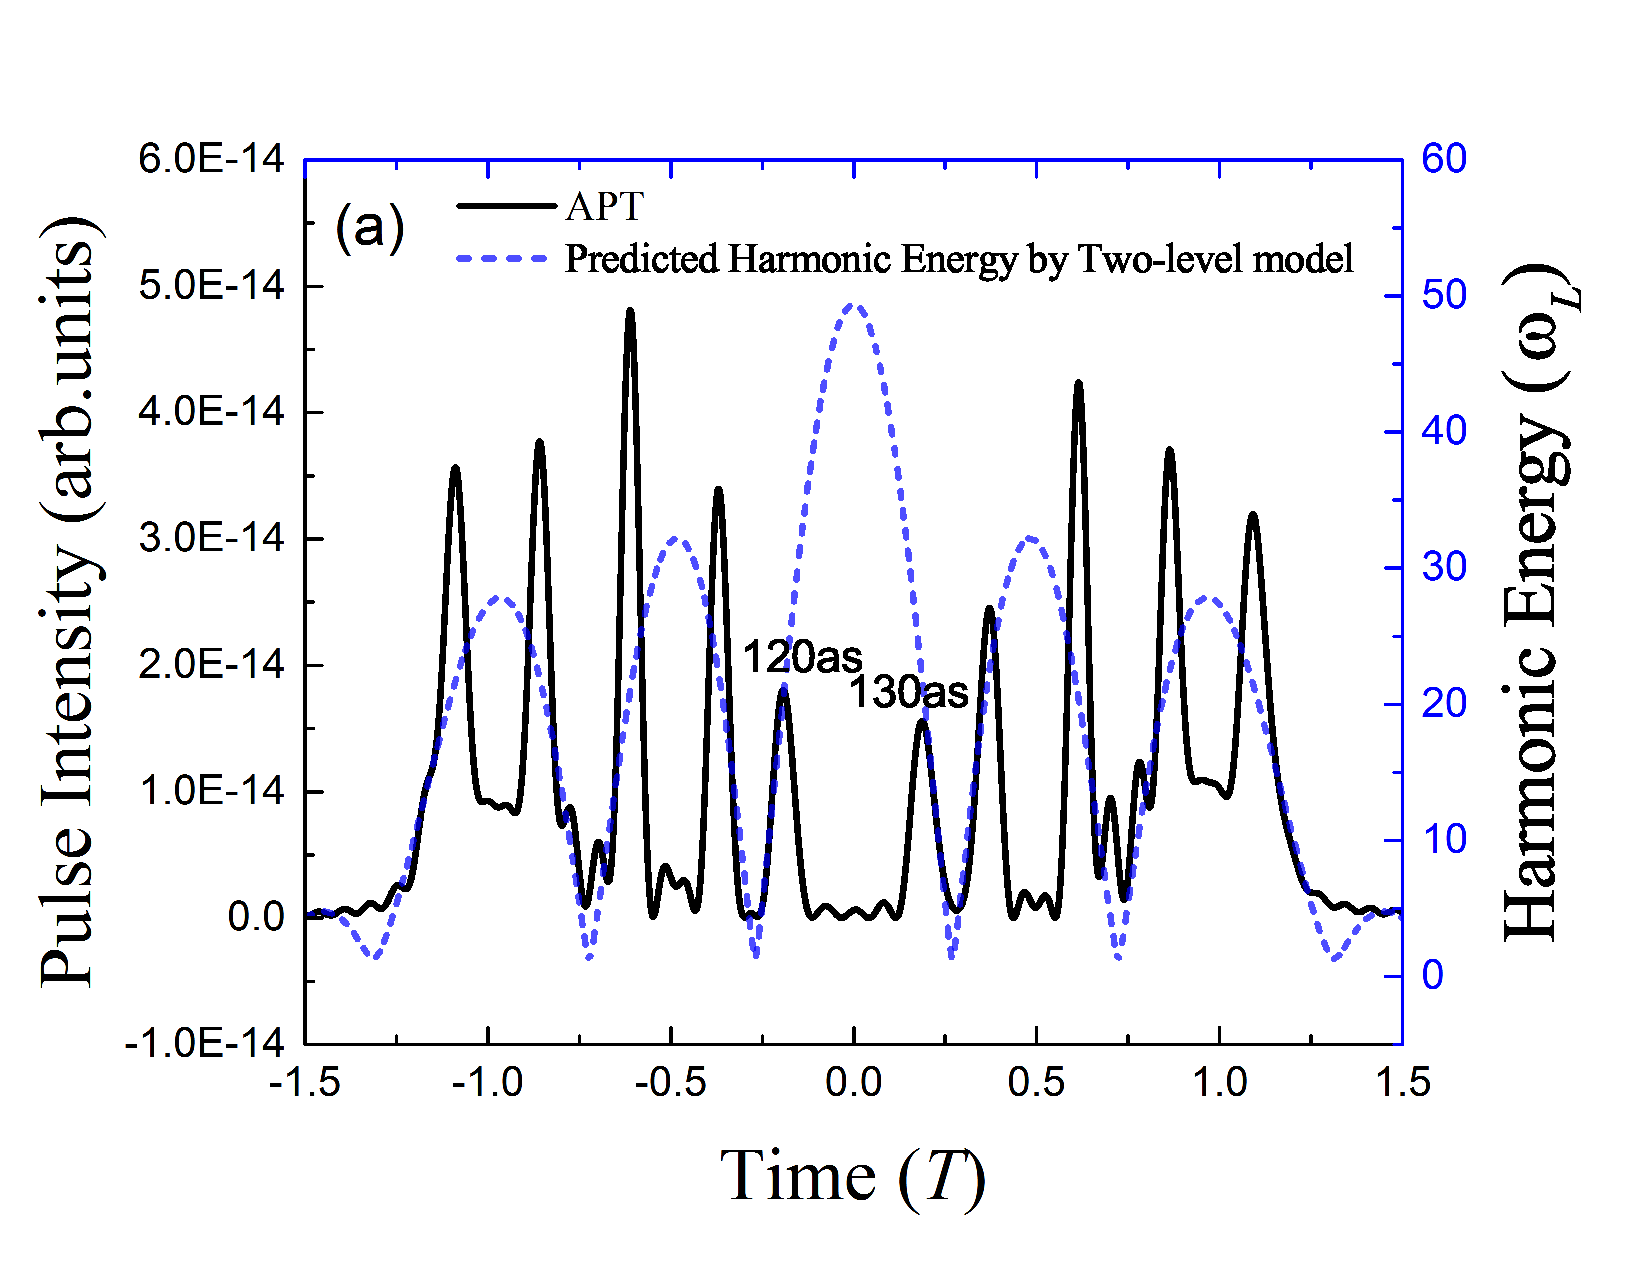
\includegraphics[width=0.4\textwidth]{fig3a.eps}
	}
%	\hspace{0.1in}
	\subfigure{
		\label{fig3b}
		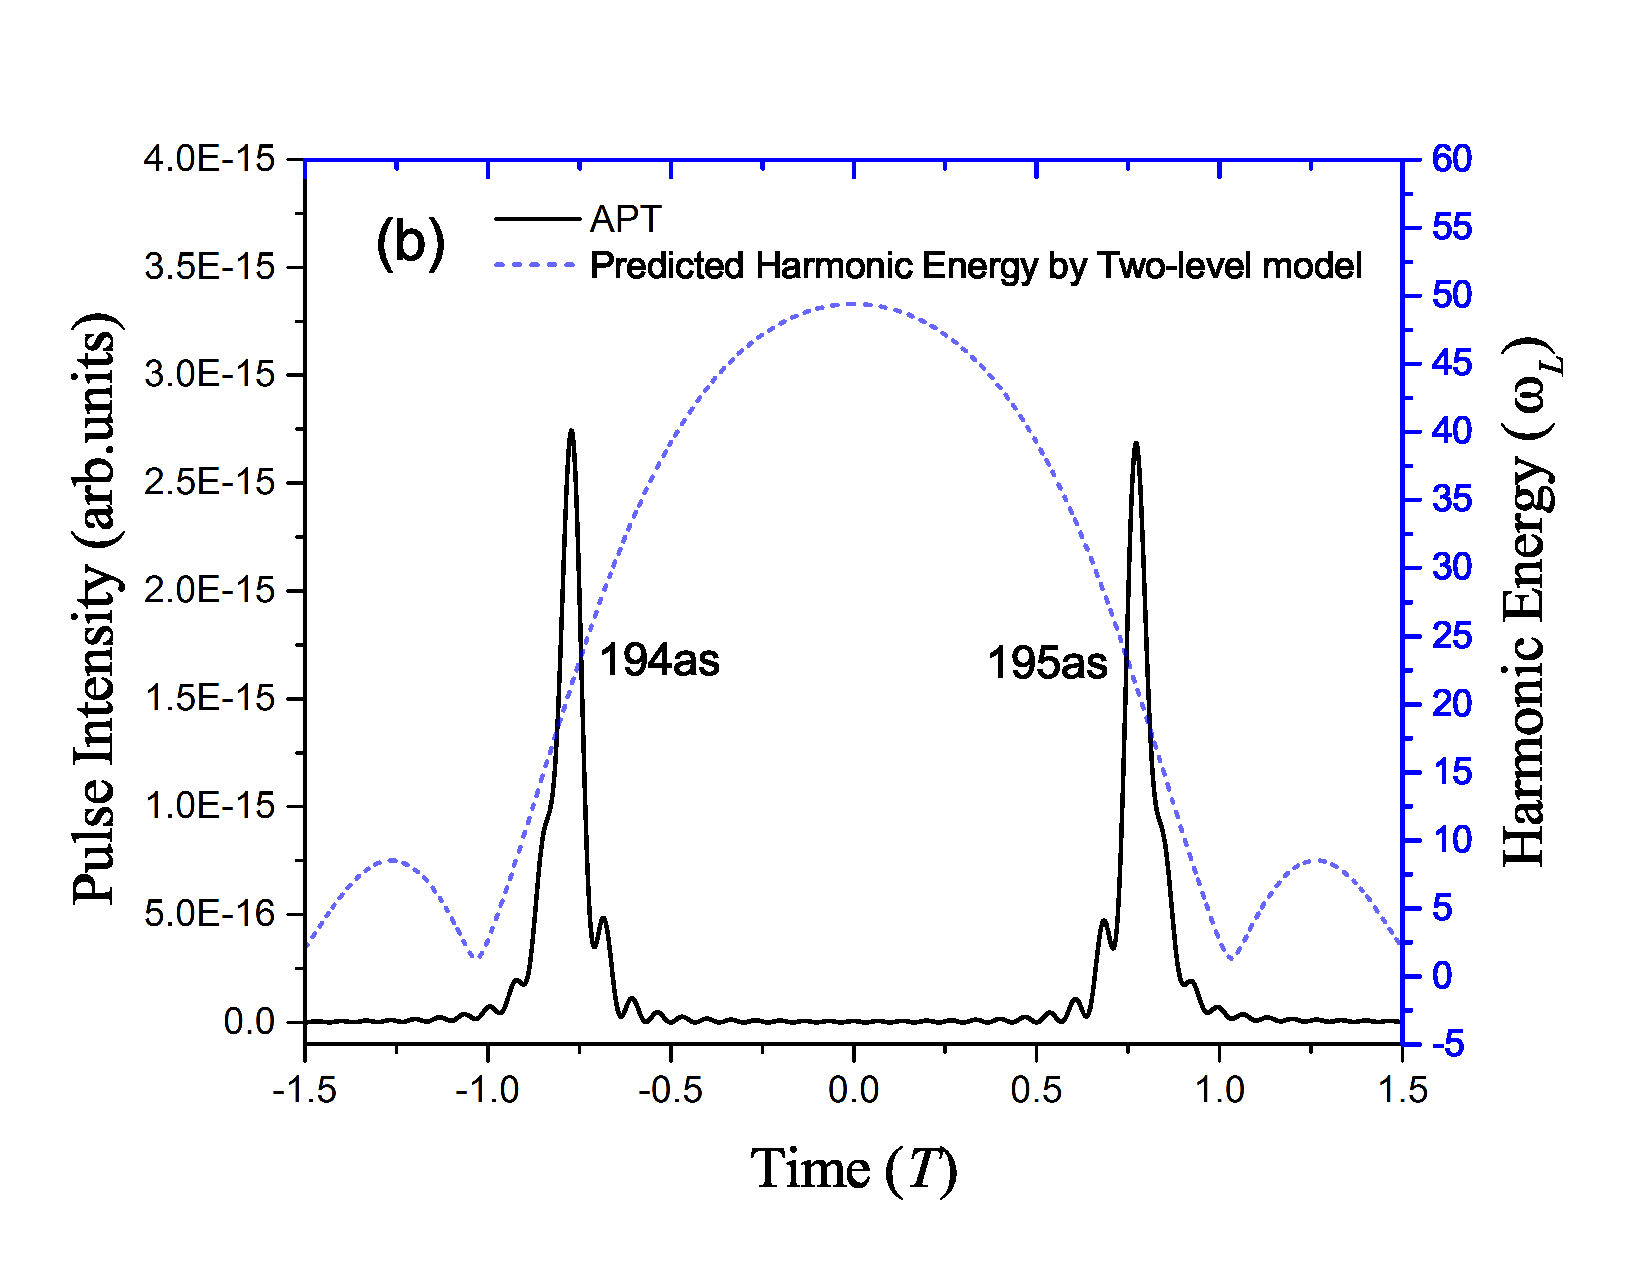
\includegraphics[width=0.4\textwidth]{fig3b.eps}
	}
	\caption{Generated (a) attosecond pulse train (APT) for without chirp case and (b) attosecond pulse pair (APP) for with chirp case by synthesizing plateau harmonics (from 14th to 29th) of driven two-level polar medium. The other laser and two-level polar medium parameters are same with those in Fig. \ref{fig2}. The blue dashed curve is the harmonic energy predicted by the two-level model ($\epsilon_{+}-\epsilon_{-}$) same with Fig. \ref{fig2c}.}
	\label{fig3}
\end{figure}
	
Thus we have demonstrated that the combination of controls, introduce of permanent dipole moment to two-level system and chirp frequency to driving laser pulse, has big influences on the HHG and attosecond pulse generation process. Due to the permanent dipole moment, much more plateau harmonics are generated and can be used to synthesize a shorter attosecond pulse; on the other hand, the chirp frequency could reduce the quantum trajectory numbers of plateau harmonics to a minimum of two which can finally lead to an APP generated. However, the pulse intensity is much weaker than that of the case without chirp (seen in Fig. \ref{fig3}). In view of this, a solution that could enhance the harmonic signal intensity should be proposed to make up the intensity loss for introducing the chirp frequency. In the following, we will investigate the propagation conditions and expect it can enhance the harmonic intensity. 
\subsection{propagation situation}
Except considering the medium relaxation time, the other medium and all the laser parameters are all the same with those of non-propagation cases as in Fig. \ref{fig3}. Initial condition of the laser pulse was given in part \emph{theoretical models and methods}. 

\begin{figure}[!htbp]
\centering
	\subfigure{
		\label{fig4a}
		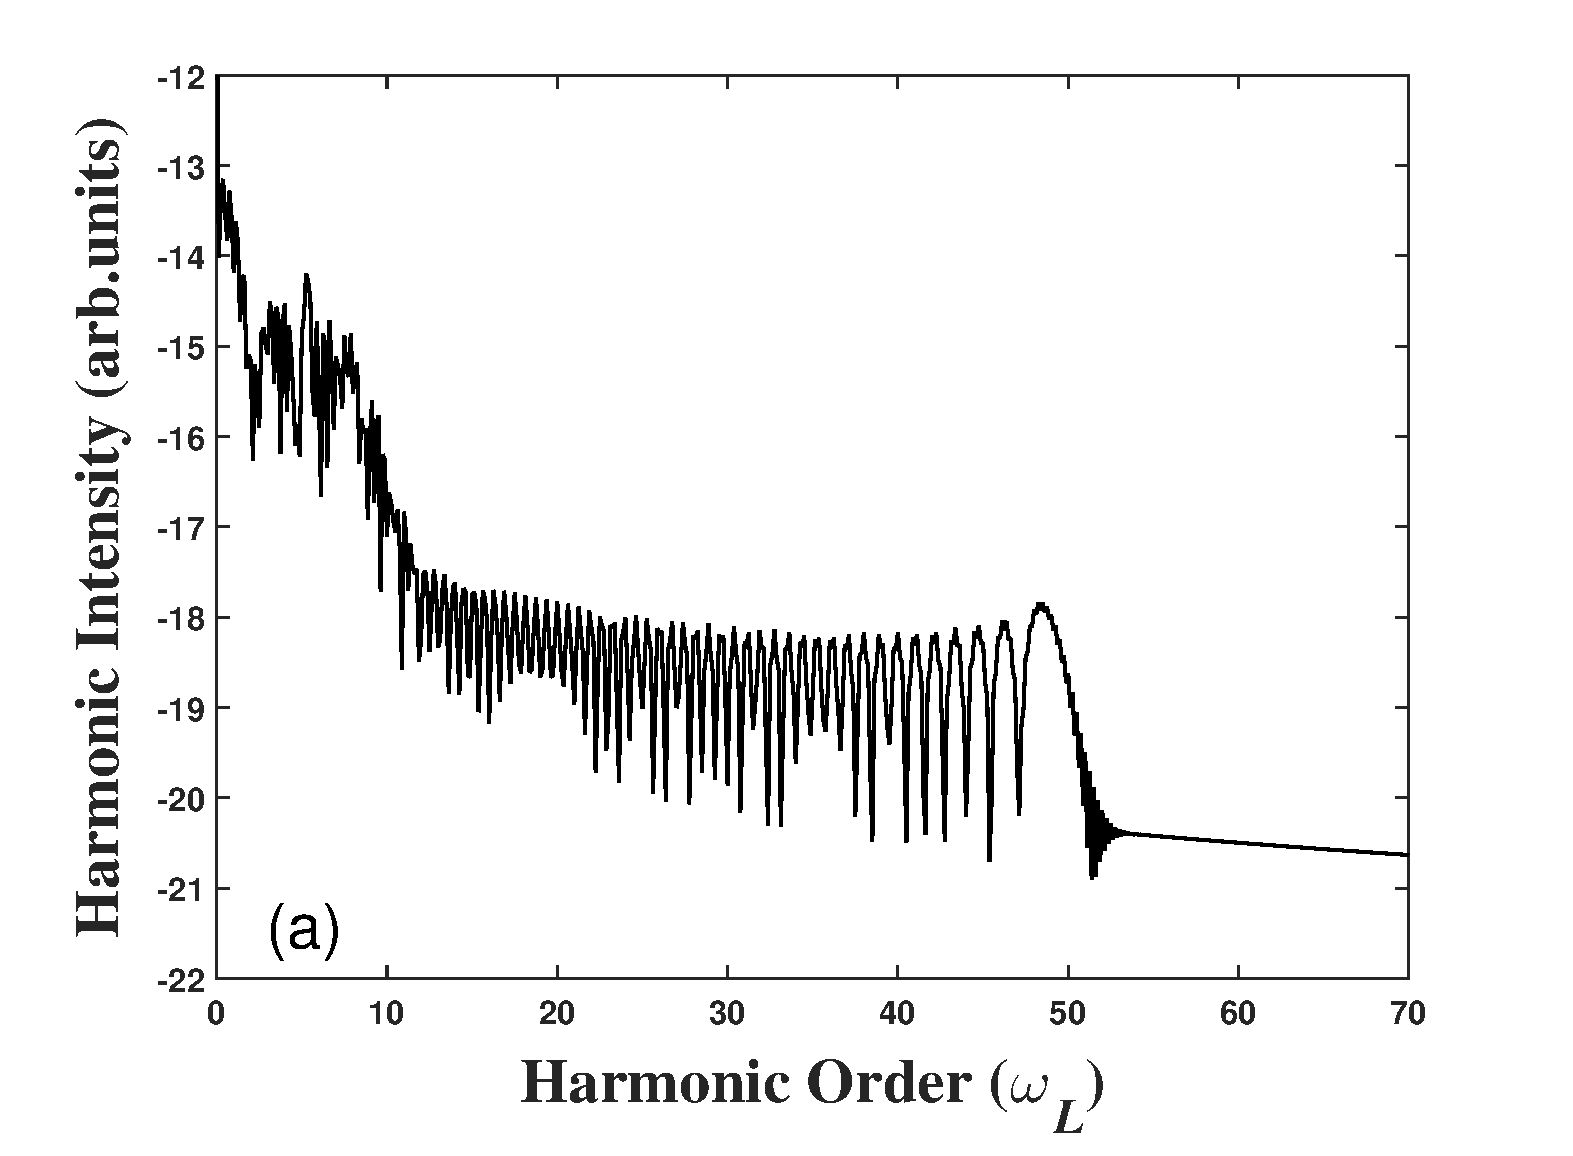
\includegraphics[width=0.45\textwidth]{fig4a.eps}
	}
	\hspace{-0.3in}
	\subfigure{
		\label{fig4b}
		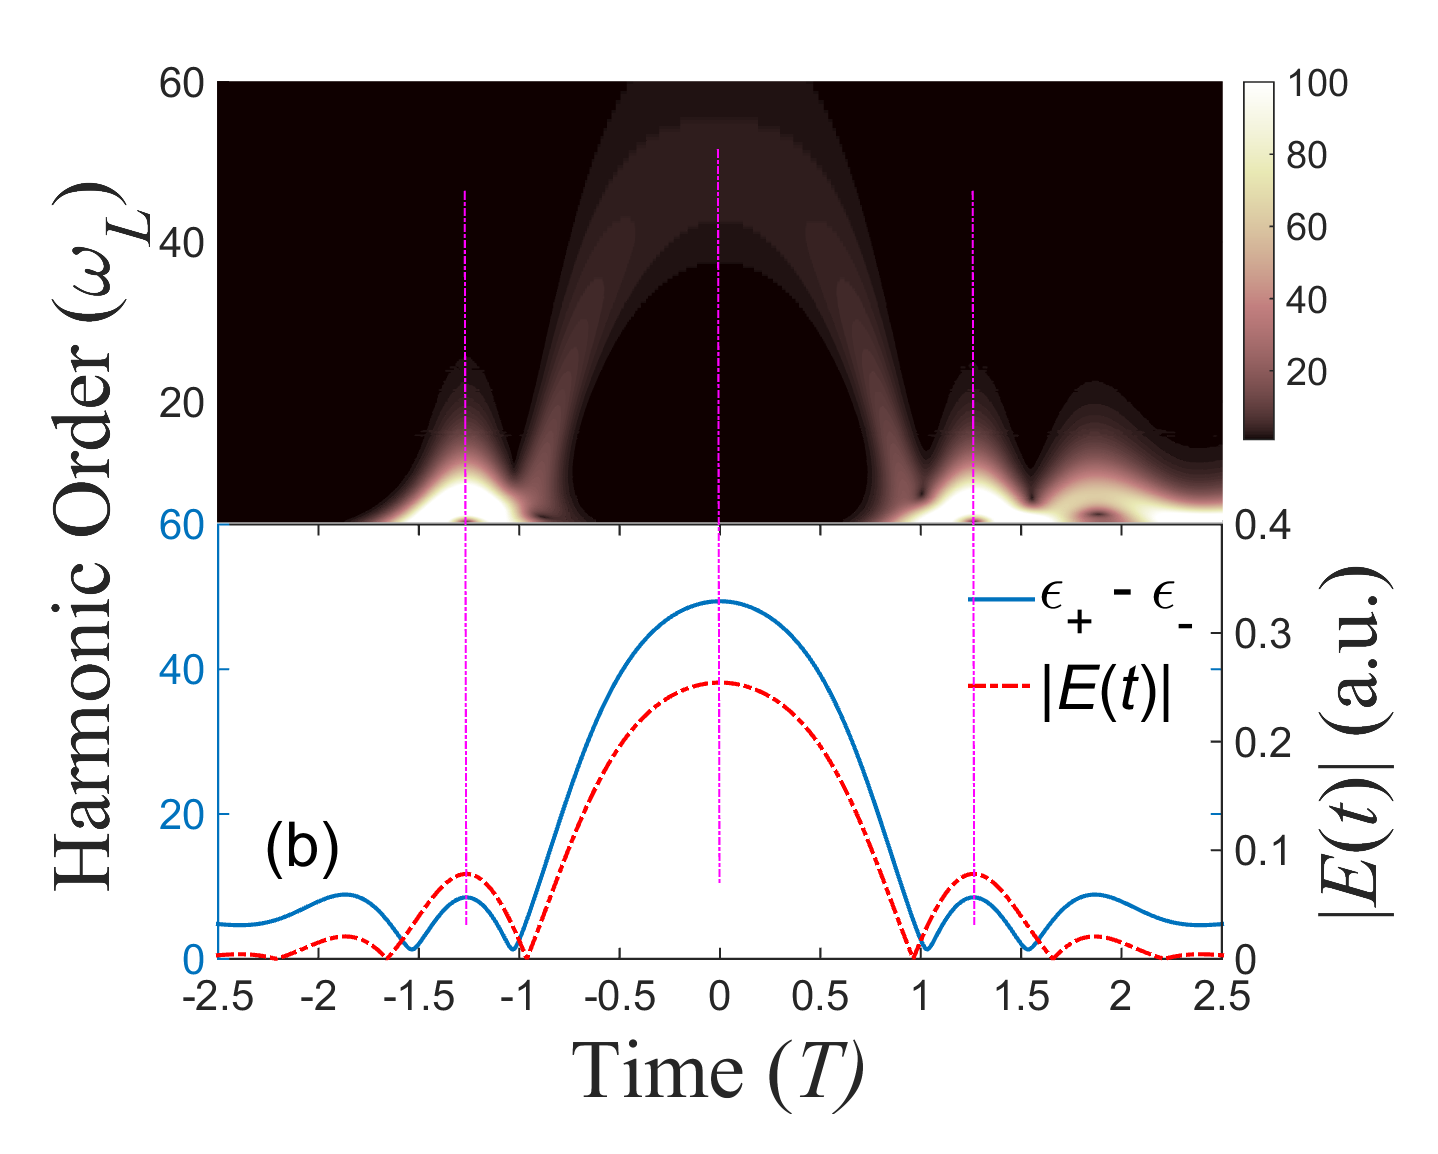
\includegraphics[width=0.45\textwidth]{fig4b.eps}
	}
	\subfigure{
		\label{fig4c}
		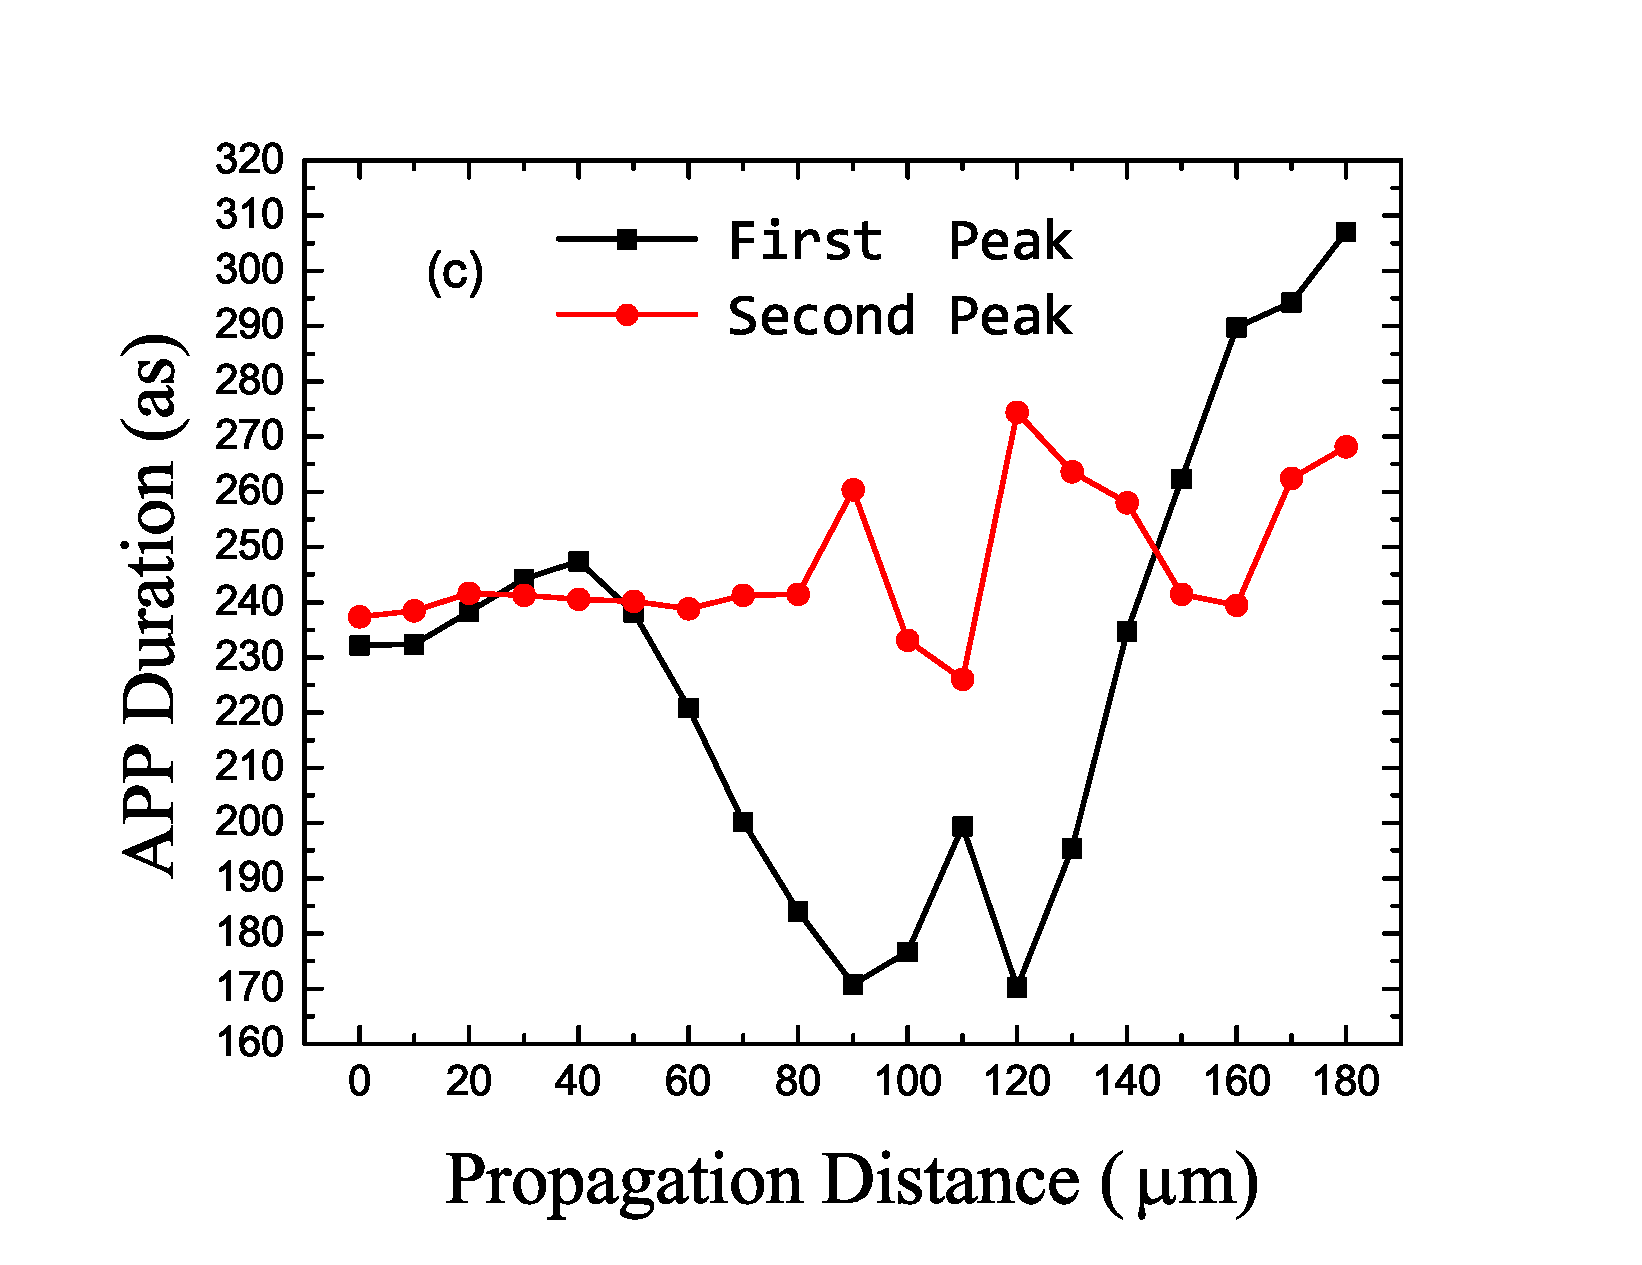
\includegraphics[width=0.45\textwidth]{fig4c.eps}
	}
	\hspace{-0.3in}
	\subfigure{
		\label{fig4d}
		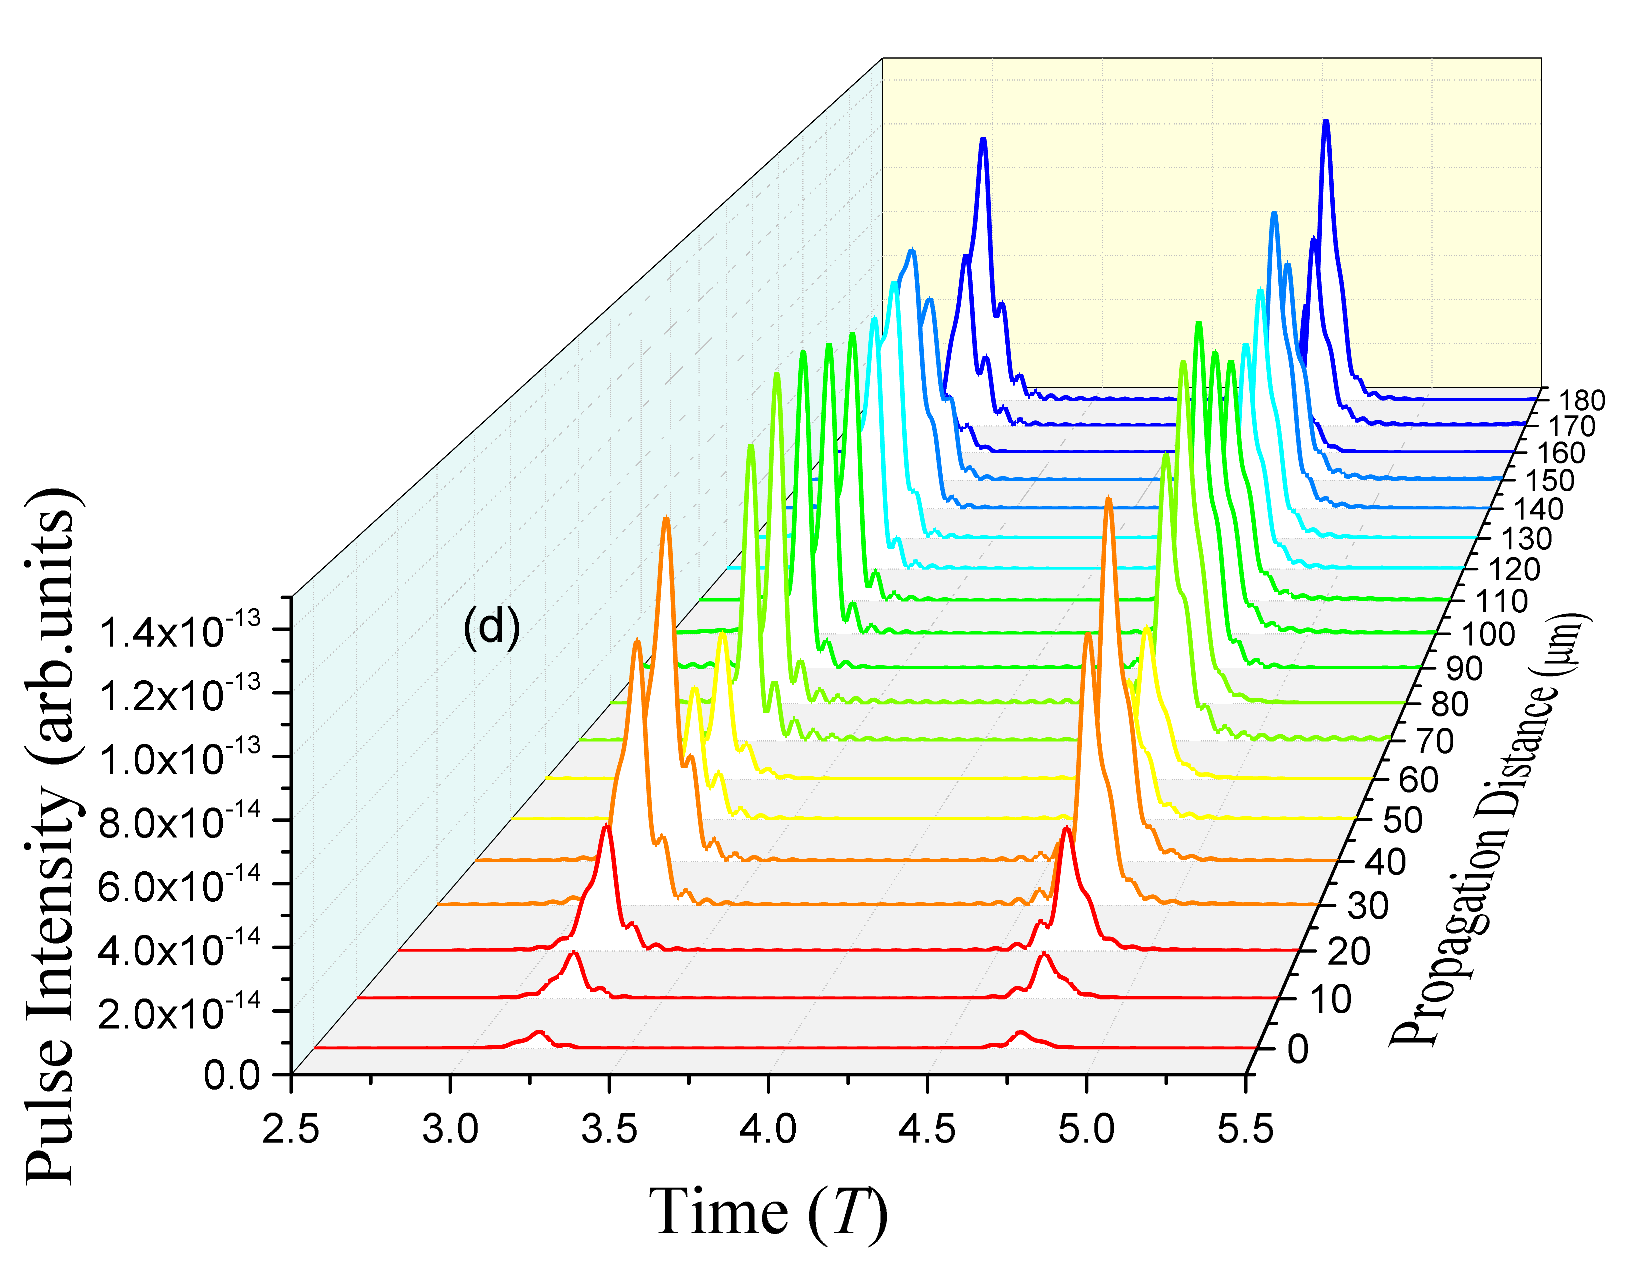
\includegraphics[width=0.45\textwidth]{fig4d.eps}
	}
\caption{(a) HHG spectra after different propagation distances. (b) Generated APPs by synthesizing plateau harmonics (between 14th to 29th) of spectra (a). (c) APP duration in a function of propagation distance. (d) Same as that in (b) but with a larger media density of $\bar{N}=12.5\times10^{24} \textrm{m}^{-3}$. Two-level system has a permanent dipole moment of $\mu_{11}=4,\;\mu_{22}=-4(\xi=-4)$. The other parameters are same with those of Fig. \ref{fig3}.}
\label{fig4}
\end{figure}

Nineteen groups of propagation distance are investigated from 0 to 180 $ \mu $m evenly divided by 10 $ \mu $m, and harmonic generation in the transmission interface will be studied, respectively. The simulation results are shown in Fig. \ref{fig4}, including the HHG spectra, generated APPs, and the APP durations. The same plateau harmonic orders (14th to 29th) are selected to synthesize the APP as Fig. \ref{fig3b}. The HHG spectra demonstrated that the propagation distance has a big influence on the plateau harmonic intensity. However the intensity is not linearly changed with propagation distance. The inset in Fig. \ref{fig4a} shows that at first the plateau harmonic intensity gradually increase to a maximum value, then decrease to a minimum value, after that it will process another increase and decrease process and so on. This process can be verified in Fig. \ref{fig4b} which clearly shows that the generated APP's intensity oscillates with propagation distance change. In our simulations, the maximum values appear at $60\mu\textrm{m}$ and $130\mu\textrm{m}$. They are about ten times that of the non-propagation case. The duration is studied for two peaks of each APP, and it also changes with propagation distance variation. The change range is about $140\textrm{as}$ from $170\textrm{as}$ to $310\textrm{as}$ in our simulations. The minimum duration value $170\textrm{as}$ appears at about $120\mu\textrm{m}$. We note that, for distances $60\mu\textrm{m}$ and $130\mu\textrm{m}$, their pulse peaks’ durations have an average about $220\textrm{as}$ which is not much longer than that of the non-propagation case. Therefore, we demonstrated that it can dramatically enhance the plateau harmonic intensity with almost no duration broadening if propagates a suitable distance in the media. In addition to this, the medium density is also studied. We increased it to $\bar{N}=12.5\times10^{24}\textrm{m}^{-3}$, and the corresponding APPs are shown in Fig. \ref{fig4d}. It shows that the maximum intensity values appear at about $40\mu\textrm{m}$, $90\mu\textrm{m}$ and $140\mu\textrm{m}$. The distance between adjacent is about $50\mu\textrm{m}$. It is about $20\mu\textrm{m}$ less than that of the case of smaller media density $\bar{N}=7.5\times10^{24}\textrm{m}^{-3}$. Therefore, one can enhance the harmonic intensity by using more dense media to propagate a shorter distance or using less dense media to propagate a longer distance alternatively.

%\begin{table}[!htbp]
%	\centering
%	\caption{Statistics for the isolated attosecond pulse's peak intensity and FWHM for the two cases of with and without chirp.}
%\begin{tabular}{cccccc}
%	\hline
%	Propagation & \multicolumn{2}{c}{Laser pulse without chirp} &  & \multicolumn{2}{c}{Laser pulse with chirp}\tabularnewline
%	\cline{2-3} \cline{5-6}
%	distance ($\mu m$) & Peak intensity (arb.units) & FWHM (as) &  & Peak intensity (arb.units) & FWHM (as)\tabularnewline
%	\hline
%	10 & 0.32 & 325 && 0.03 & 950\tabularnewline
%	20 & 0.25 & 325 && 0.03 & 950\tabularnewline
%	30 & 0.19 & 300 && 0.06 & 980\tabularnewline
%	40 & 0.14 & 300 && 0.11 & 950\tabularnewline
%	50 & 0.13 & 300 && 0.22 & 950\tabularnewline
%	60 & 0.23 & 300 && 0.36 & 980\tabularnewline
%	70 & 0.46 & 300 && 0.48 & 950\tabularnewline
%	80 & 0.48 & 300 && 0.51 & 950\tabularnewline
%	90 & 0.09 & 300 && 0.44 & 950\tabularnewline
%	\hline
%\end{tabular}
%	\label{table1}

%\end{table}

\section{Conclusions}
In this paper, we have tried to combine the control of the matter and the control of the driving laser pulse to produce a high-order harmonic spectrum with a higher cutoff energy. It is shown that the existence of the permanent dipole moments can significantly extend the plateau of the harmonic spectrum. However, the plateau harmonic has more than two quantum trajectories, which can not generate an IAP by synthesizing harmonics within this region. If the laser pulse is chirped, its oscillatory periodicity and up-down symmetry will be dramatically changed. This kind of laser pulse can exactly reduce the quantum trajectory number to a minimum of two. There's still no an IAP generated, but an APT with only two individual peaks (APP) is obtained. If the propagation effect is considered, it can dramatically enhance the APP intensity (maximum by one order) for a suitable propagation distance with almost no duration broadening.

\section*{Acknowledgments}
This work is supported by the National Natural Science Foundation of China (NNSF, Grant
No.11374318). C.L. appreciates the supports from the 100-Talents Project of Chinese Academy
of Sciences and Department of Human Resources and Social Security of China.

\end{document}

